%%%%%%%%%%%%%%%%%%%%%%%%%%%%%%%%%%%%%%%%%%%%%%%%%%%%%%%%%%%%%%%%%%%%%%%%%%%%%%%%%%%%%%%%%%%%%%%%%%%%%%%%%%%%%%%%%%%%%%%%%%%%%%%%%%%%%%%%%%%%%%%%%%%%%%%%%%%
% This is just an example/guide for you to refer to when submitting manuscripts to Frontiers, it is not mandatory to use Frontiers .cls files nor frontiers.tex  %
% This will only generate the Manuscript, the final article will be typeset by Frontiers after acceptance.   
%                                              %
%                                                                                                                                                         %
% When submitting your files, remember to upload this *tex file, the pdf generated with it, the *bib file (if bibliography is not within the *tex) and all the figures.
%%%%%%%%%%%%%%%%%%%%%%%%%%%%%%%%%%%%%%%%%%%%%%%%%%%%%%%%%%%%%%%%%%%%%%%%%%%%%%%%%%%%%%%%%%%%%%%%%%%%%%%%%%%%%%%%%%%%%%%%%%%%%%%%%%%%%%%%%%%%%%%%%%%%%%%%%%%

%%% Version 3.4 Generated 2018/06/15 %%%
%%% You will need to have the following packages installed: datetime, fmtcount, etoolbox, fcprefix, which are normally inlcuded in WinEdt. %%%
%%% In http://www.ctan.org/ you can find the packages and how to install them, if necessary. %%%
%%%  NB logo1.jpg is required in the path in order to correctly compile front page header %%%

\documentclass[utf8]{frontiersSCNS} % for Science, Engineering and Humanities and Social Sciences articles
%\documentclass[utf8]{frontiersHLTH} % for Health articles
%\documentclass[utf8]{frontiersFPHY} % for Physics and Applied Mathematics and Statistics articles

%\setcitestyle{square} % for Physics and Applied Mathematics and Statistics articles
%\usepackage{url,hyperref,lineno,microtype,subcaption}
\usepackage{url,hyperref,lineno,microtype}
\usepackage[onehalfspacing]{setspace}

\linenumbers


% Leave a blank line between paragraphs instead of using \\


\def\keyFont{\fontsize{8}{11}\helveticabold }
\def\firstAuthorLast{Treder} %use et al only if is more than 1 author
\def\Authors{Matthias S. Treder}
% Affiliations should be keyed to the author's name with superscript numbers and be listed as follows: Laboratory, Institute, Department, Organization, City, State abbreviation (USA, Canada, Australia), and Country (without detailed address information such as city zip codes or street names).
% If one of the authors has a change of address, list the new address below the correspondence details using a superscript symbol and use the same symbol to indicate the author in the author list.
\def\Address{School of Computer Science \& Informatics, Cardiff University, Cardiff, UK}
% The Corresponding Author should be marked with an asterisk
% Provide the exact contact address (this time including street name and city zip code) and email of the corresponding author
\def\corrAuthor{Corresponding Author}

\def\corrEmail{trederm@cardiff.ac.uk}

%%% --- added by Matthias ---
\usepackage{tabularx}  % controls the table width
\usepackage{prettyref}
\usepackage{amsmath}
\usepackage{xcolor}
\usepackage{bbm}    % for 1 as a vector

\newtheorem{theorem}{Theorem}

% Math symbols
\newcommand{\al}{\boldsymbol{\alpha}}
\newcommand{\m}{\mathbf{m}}
\newcommand{\mf}[2]{m_#1^{(#2)}}
\newcommand{\mbar}{\overline{\m}}
\newcommand{\mm}[1]{\m_{#1}}
\newcommand{\sig}[2]{(\sigma^2)_#1^{(#2)}}
\newcommand{\w}{\mathbf{w}}
\newcommand{\x}{\mathbf{x}}
\newcommand{\xf}[1]{\mathbf{x}^{(#1)}} % x features
\newcommand{\y}{\mathbf{y}}
\newcommand{\cov}{\text{cov}}
\newcommand{\C}{\mathbf{C}}
\newcommand{\E}{\mathbb{E}}   % expectation
\newcommand{\G}{\mathbf{G}}
\newcommand{\I}{\mathbf{I}}
\newcommand{\K}{\mathbf{K}}
\renewcommand{\L}{\mathcal{L}}
\newcommand{\M}{\mathbf{M}}
\newcommand{\N}{\mathcal{N}}   % normal distribution
\newcommand{\Q}{\mathbf{Q}}
\newcommand{\R}{\mathbb{R}}
\renewcommand{\S}{\mathbf{S}}
\newcommand{\Tr}[1]{\text{Tr}(#1)}
\newcommand{\W}{\mathbf{W}}
\newcommand{\X}{\mathbf{X}}
\newcommand{\Y}{\mathbf{Y}}

\newcommand{\ttt}[1]{\texttt{#1}}

\newrefformat{fig}{Figure \ref{#1}}
\newrefformat{tab}{Table \ref{#1}}
\newrefformat{eq}{Eq. (\ref{#1})}
\newrefformat{app}{Appendix \ref{#1}}
\newrefformat{sec}{Section \ref{#1}}
\newrefformat{lemma}{Lemma \ref{#1}}
\newrefformat{theorem}{Theorem \ref{#1}}
\newrefformat{assumption}{Assumption \ref{#1}}

\newcommand{\red}[1]{\textcolor{red}{#1}}
\newcommand{\todo}[1]{\textcolor{red}{\textbf{todo} #1}}

\graphicspath{{../figures/}}


\begin{document}
\onecolumn
\firstpage{1}

%\title[MVPA-Light]{MVPA-Light: out-of-the-box classification of neuroimaging data}
%\title[MVPA-Light]{MVPA-Light: a classification suite for neuroimaging data}
\title[MVPA-Light]{MVPA-Light: a classification and regression toolbox for multi-dimensional data}

\author[\firstAuthorLast ]{\Authors} %This field will be automatically populated
\address{} %This field will be automatically populated
\correspondance{} %This field will be automatically populated

\extraAuth{}% If there are more than 1 corresponding author, comment this line and uncomment the next one.
%\extraAuth{corresponding Author2 \\ Laboratory X2, Institute X2, Department X2, Organization X2, Street X2, City X2 , State XX2 (only USA, Canada and Australia), Zip Code2, X2 Country X2, email2@uni2.edu}


\maketitle


\begin{abstract}

%%% Leave the Abstract empty if your article does not require one, please see the Summary Table for full details.
\section{}
MVPA-Light is a MATLAB toolbox for multivariate pattern analysis (MVPA). It provides native implementations of a range of classifiers (LDA, Logistic Regression, SVM, kernel FDA, Naive Bayes, ensemble methods) and regression models (ridge, kernel ridge), using modern optimization algorithms. High-level functions allow for the multivariate analysis of multi-dimensional data, including generalization (e.g. time x time) and searchlight analysis. The toolbox performs  cross-validation, hyperparameter tuning, and nested preprocessing. It computes various classification and regression metrics and establishes their statistical significance. It is modular, easily extendable, and is shipped with sample data and example scripts. Furthermore, it offers interfaces for LIBSVM and LIBLINEAR as well as an integration into the FieldTrip neuroimaging toolbox.



\tiny
 \keyFont{ \section{Keywords:} toolbox, classification, decoding, MVPA, SVM, Linear Discriminant Analysis, Logistic Regression, ridge regression, kernel methods, ensemble methods, regularization, cross-validation
 } %All article types: you may provide up to 8 keywords; at least 5 are mandatory.
\end{abstract}

%%% -------- INTRODUCTION --------
\section{Introduction}

During the early 2010s, multivariate pattern analysis (MVPA) became a mainstream statistical tool in EEG/MEG research \citep{Blankertz2011,Lemm2011,Mur2009,Grootswagers2017DecodingData,Pereira2009,Varoquaux2017}. It can be considered as a complement to the set of traditional statistical tools available to researchers (e.g. t-test, ANOVA). MVPA is particularly suited to large, multivariate datasets. Furthermore, since many classifiers make few or no assumptions about the data distribution, and statistical significance is often established using permutation tests, MVPA can be considered as a set of non-parametric statistical tools.
One of the primary applications of MVPA is \textit{classification}. In classification, an algorithm called \textit{classifier} takes a multivariate pattern of brain activity (referred to as \textit{features}) as input and maps it onto a categorical brain state or experimental condition (referred to as \textit{class label}). In other words, the task of a classifier is to predict class labels given features. The terms classification/classifier are also known as decoding/decoder in the cognitive neuroscience literature. It is worth noting that classification is often performed at the level of individual participants, taking trials as data samples. The classifier output then corresponds to predictions for single trials. \red{Another important application of MVPA is \textit{regression}. It shares many characteristics with classification, but it uses a \textit{regression model} to map features onto a continuous variable (e.g. reaction time) referred to a \textit{responses}. Consequently, predictions of the regression model are continuous  (e.g. predicted reaction time given a brain pattern).}

A number of excellent MATLAB toolboxes for MVPA have been developed over the years, including the Berlin BCI toolbox \citep{Blankertz2016TheControl}, Amsterdam Decoding and Modelling Toolbox (ADAM) \citep{Fahrenfort2018FromADAM}, BCILAB \citep{Kothe2013BCILAB:Development}, Donders Machine Learning Toolbox (DMLT) (\texttt{github.com/distrep/DMLT}), Decision Decoding ToolBOX (DDTBOX) \citep{Bode2019ThePotentials}, Pattern Recognition for Neuroimaging Toolbox (PRoNTo) \citep{Schrouff2013PRoNTo:Toolbox}, and CoSMoMVPA \citep{Oosterhof2016CoSMoMVPA:Octave}. Beyond MATLAB, the probably most popular computer languages for machine learning are Python and R, with outstanding toolboxes such as Scikit-learn \citep{Pedregosa2011Scikit-learn:Python} for Python and Caret \citep{Kuhn2008BuildingPackage} and MLR \citep{Bischl2000Mlr:R} for R. A comprehensive comparison of MVPA-Light with all these toolboxes is beyond the scope of this paper, but we believe that what sets MVPA-Light apart is the adherence to all of the following design principles: 

\begin{itemize}
\item \textit{self-contained}: unlike many toolboxes that provide wrappers for existing classifiers, the backbone of MVPA-Light is  native implementations of various classifiers (LDA, kernel FDA, Logistic Regression, SVM, Naive Bayes and ensemble methods), regression models, and their corresponding optimization algorithms (Trust-Region Newton, Dual Coordinate Descent). As a result, MVPA-Light works out-of-the-box, without the need for additional toolboxes or  code compilation.
\item \textit{transparent}: the toolbox has a shallow code base with well-documented functions. In many cases, the function call stack has a depth of two within the toolbox. For instance, a call to \texttt{mv\_crossvalidate} using an LDA classifier triggers calls to functions such as  \texttt{mv\_check\_inputs}, \texttt{train\_lda} and \texttt{test\_lda}. Although the train/test functions might call additional optimization functions, most of the work is done at these two shallowest levels. To preserve the shallowness, high-level functions replicate some code that might be shared otherwise. Furthermore, object orientation and encapsulation is avoided in favour of the more transparent MATLAB structs.
\item \textit{fast}: all models and high-level functions are written with speed as a prime concern. In some cases, the need for speed conflicts with the out-of-the-box requirement. For instance, Logistic Regression and SVM use iterative optimization algorithms written in MATLAB. However, these algorithms run substantially faster using compiled code. To this end, an interface is provided for LIBSVM \citep{Chang2011LIBSVM:Machines} and LIBLINEAR \citep{Fan2008}, two excellent C implementations of Logistic Regression and SVM for users who do not shy away from compiling the code on their platform.
\item \textit{modular and pluggable}: it is possible, and intended, to harvest parts of the code such as the classifiers for other purposes. It is also easy to plug the toolbox into a larger EEG/MEG processing framework. An interface for FieldTrip \citep{Oostenveld2011} is described in the Methods section.
\item \textit{high-level interface}: common MVPA tasks such as searchlight analysis and time generalization including cross-validation can be performed with a few lines of MATLAB code. Many of the hyperparamaters required by classifiers and regression models can be set to 'auto'; the parameters are then automatically selected by MVPA-Light, taking the burden of hyperparameter selection off the user. For an effortless start, a small EEG dataset and example scripts are shipped with the toolbox.
\end{itemize}

It is worth noting that MVPA-Light is a purely statistical toolbox. That is, it assumes that data has been preprocessed with a neuroimaging toolbox and comes in the shape of MATLAB arrays. Many toolboxes (e.g. FieldTrip, SPM, EEGLAB) store the imaging  data in such arrays, so that MVPA-Light can easily be used as a plugin tool. This comes with the perk that adaptation to other imaging modalities such as NIRS and fMRI is straightforward.

\subsection{Getting started}

MVPA-Light is shipped with a set of example scripts (in the \ttt{/examples} subfolder) and an example EEG dataset. These scripts cover both the high-level functions in MVPA-Light and calling the train/test functions manually. The best starting point is to work through the example scripts and then adapt them to one's purpose. An up-to-date introduction to the toolbox with relevant hyperlinks is provided on the GitHub page (\ttt{github.com/treder/mvpa-light}).

The EEG data has been taken from the free BNCI-Horizon-2020 data repository (http://bnci-horizon-2020.eu/database). It consists of three \ttt{mat} files corresponding to three subjects (subject codes \ttt{VPaak}, \ttt{VPaan}, and \ttt{VPgcc}) from the auditory oddball dataset introduced in \cite{Treder2014}. Out of the experimental conditions, the "SynthPop" condition has been selected. Attended and unattended deviants are coded as class 1 and 2. The 64 EEG channels in the original dataset have been reduced to 32 channels.

To give a concrete code example, consider a [samples x channels] data matrix for one participant, where the samples correspond to trials and the channels serve as features. The matrix is denoted as \ttt{X}. Each trial corresponds to either condition 1 (e.g. oddball sound) or condition 2 (standard sound). This is encoded in a vector of class labels, denoted as \ttt{clabel}, that contains 1's and 2's. Then the following piece of code performs 10-fold cross-validation with 2 repetitions. LDA is used as classifier and area under the ROC curve (AUC) is calculated as a classification metric.

\begin{verbatim}
cfg = [];
cfg.classifier = 'lda';
cfg.metric     = 'auc';
cfg.cv         = 'kfold';
cfg.k          = 10;
cfg.repeat     = 2;

perf = mv_crossvalidate(cfg, X, clabel);
\end{verbatim}

The output value \ttt{perf} contains the classifier performance measure, in this case a single AUC value averaged across test folds and repetitions. \ttt{mv\_crossvalidate} is part of the high-level interface that will be discussed next.

In the next section, the toolbox will be described in more detail and an classification analysis based on a publicly available MEEG dataset will be reported upon \citep{Wakeman2014OpenfMRI,Wakeman2015ADataset}.

%%% ------------------------
%%% ------------------------
%%% -------- METHOD --------
%%% ------------------------
%%% ------------------------
\section{Materials and methods}

\red{\subsection{Requirements}}

A standard Desktop or Laptop is sufficient to run MVPA-Light. The memory requirement is dictated by the memory footprint  of the dataset. Since some functions operate on a copy of the data, it is recommended that the available RAM exceeds the size of the dataset by at least a factor of two (e.g. 4+ GB RAM for a 2 GB dataset). MVPA-Light is supported by MATLAB 2012a and more recent versions. The Statistics toolbox is required at some points in the toolbox (e.g. for calculating t-values). The cluster permutation test in \ttt{mv\_statistics} uses the Image Processing toolbox to extract the clusters.

%%% -----------------------------
%%% --- HIGH-LEVEL FUNCTIONS ----
%%% -----------------------------
\subsection{High-level interface}

The structure of the toolbox is depicted in \prettyref{fig:structure}. 
The toolbox can be interacted with through high-level functions that cover many common classification tasks. \ttt{mv\_crossvalidate} performs a single cross-validation analysis on a 2-D [samples $\times$ features] dataset \ttt{X}. The next two functions, \ttt{mv\_classify\_across\_time}  and \ttt{mv\_classify\_timextime}, assume that the data has a time dimension as well, i.e. it is a 3-D [samples $\times$ features $\times$ time points] array. \ttt{mv\_classify\_across\_time} performs classification for every time point, resulting in a vector of cross-validated metrics (e.g. accuracy), the length of the vector being the number of time points. In contrast, \ttt{mv\_classify\_timextime} implements time generalization \citep{King2014}, that is, classification for every combination of training and test time points, resulting in a 2-D matrix of cross-validated metrics. \ttt{mv\_searchlight}  performs classification for every feature (e.g. EEG channels) separately, resulting in a vector of cross-validated metrics, the length of the vector being the number of features (e.g. channels). This is useful for identifying the spatial location of discriminative information. Lastly, \ttt{mv\_classify} is a more general-purpose function that works on data of arbitrary dimension (e.g. time-frequency data). It combines the capabilities of all the other high-level functions at the expense, to some extent, of ease and speed. \red{For regression tasks, the equivalent to \ttt{mv\_classify} is the function \ttt{mv\_regress}. It also works with data of arbitrary dimension and supports both searchlight and generalization.}

All high-level functions take three input arguments. First, \ttt{cfg}, a configuration structure wherein parameters for the analysis can be set. Second, \ttt{X}, the EEG/MEG data acting as input to the classifier. Third, \ttt{clabel}, a vector of class labels representing a numerical encoding of discrete brain states or experimental conditions. Some of the parameters in the \ttt{cfg} struct are common  to all high-level functions:

\begin{itemize}
    \item \ttt{cfg.hyperparameter}: a substruct that specifies the hyperparameters for the classifier. For instance, \ttt{cfg.hyperparameter.lambda = 0.1} sets the magnitude of shrinkage regularization in LDA.
    \item \ttt{cfg.metric}: specifies the metric to be calculated from the classifier outputs. e.g. classification accuracy or mean-squared error for regression. Metrics are introduced in \prettyref{sec:metrics}.
    \item \ttt{cfg.preprocess}: a substruct that specifies a nested preprocessing pipeline. The pipeline consists of preprocessing operations that are applied on train and test data separately. Preprocessing is discussed in \prettyref{sec:preprocessing}.
\end{itemize}

Additionally, the \ttt{cfg} struct includes the cross-validation settings explained in the next section.


\subsubsection{Cross-validation}

To obtain a realistic estimate of classification or regression performance and control for overfitting, a model should be tested on an independent dataset that has not been used for training. In most neuroimaging experiments, there is only one dataset with a restricted number of trials. K-fold cross-validation makes efficient use of such data by splitting it into k different folds. In every iteration, one of the k folds is held out and used as test set, whereas all other folds are used for training. This is repeated until every fold served as test set once. Since cross-validation itself is stochastic due to the random assignment of samples to folds, it can be useful to repeat the cross-validation several times and average the results. See \cite{Lemm2011,Varoquaux2017} for a discussion of cross-validation and potential pitfalls. Cross-validation is implemented in all high-level functions. It is controlled by the following parameters:

\begin{itemize}
    \item \ttt{cfg.cv}: cross-validation type, either \ttt{'kfold'}, \ttt{'leaveout'}, \ttt{'holdout'} or \ttt{'none'} (default \ttt{'kfold'}).
    \item \ttt{cfg.k}: number of folds in k-fold cross-validation (default 5).
    \item \ttt{cfg.repeat}: number of times the cross-validation is repeated with new randomly assigned folds (default 5).
    \item \ttt{cfg.p}: if \ttt{cfg.cv} is \ttt{'holdout'}, \ttt{p} is the fraction of test samples (default 0.1).
    \item \ttt{cfg.stratify}: if 1, for classification, the class proportions are approximately preserved in each test fold (default 1).
\end{itemize}

\subsubsection{Hyperparameter tuning}

Hyperparameters are parameters describing a classifier or regression model that need to be specified by the user, such as the type and amount of regularization applied, the type of kernel, and the kernel width $\gamma$ for Gaussian kernels. From the user's perspective, hyperparameters can be nuisance parameters: it is sometimes not clear a priori how to set them, but their exact value can have a substantial effect on the result.

MVPA-Light tries to automate hyperparameter selection as much as possible. This is done using either reasonable default values, hyperparameter estimators (e.g., \cite{Ledoit2003HoneyMatrix} for LDA) or the use of  hyperparameter-free regularizers (log-F(1,1) for Logistic Regression). If this is not possible, automated grid search using nested cross-validation can be used for testing out different hyperparameter combinations essentially by brute force. \red{For better performance, bespoke hyperparameter tuning functions are implemented for some classifiers. Otherwise, the generic tuning function \ttt{mv\_tune\_hyperparameters} is used.}

%%% ------- PREPROCESSING -------
\subsubsection{Preprocessing}\label{sec:preprocessing}

Preprocessing refers to operations applied to the data prior to training the classifier. To not bias the result, some preprocessing operations (such as Common Spatial Patterns) should be performed in a 'nested' fashion. That is, they are performed on the training data first and subsequently applied to the test data using parameters estimated from the training data \citep{Lemm2011,Varoquaux2017}. 
Currently implemented functions include PCA, sample averaging \citep{Cichy2017MultivariateSpace}, kernel averaging \citep{Treder2018}, and under-/oversampling for unbalanced data. Preprocessing pipelines are defined by adding the \ttt{cfg.preprocess} parameter. For instance,

\begin{verbatim}
cfg.preprocess = {'undersample', 'zscore', 'average_kernel'}
\end{verbatim}

adds a preprocessing pipeline that perfoms undersampling of the data followed by z-scoring and kernel averaging.

%%% -----------------------------
%%% -------- CLASSIFIERS --------
%%% -----------------------------
\subsection{Classifiers}\label{sec:classifiers}

Classifiers are implemented using pairs of train/test functions. In the high-level functions, a classifier is selected using the \ttt{cfg.classifier} parameter. However, as a low-level interface, the train/test functions can be called directly. For instance, 

\begin{verbatim}
cf = train_lda(param, X, clabel)
\end{verbatim}

calls the train function for an LDA classifier, where \ttt{X} is the training data and \ttt{clabel} are the corresponding class labels. \ttt{param} is a MATLAB struct that contains hyperparameters. Hyperparameters are specific for each classifier. For instance, \ttt{lambda = 0.5} sets the regularization hyperparameter in LDA. In many cases, the default hyperparameters yield good results. For fine-grained control of the hyperparameters, the user can refer to the documentation of the train functions. The hyperparameters for LDA can be accessed by typing \ttt{help(train\_lda)} in MATLAB. 

The output \ttt{cf} is a struct that contains the classifier's parameters after training. For linear classifiers, \ttt{cf.w} is the weight vector specifying the linear combination of features and \ttt{cf.b} is the threshold/bias term. The classifier can be applied to test data, denoted as \ttt{Xtest}, by calling

\begin{verbatim}
[clabel, dval, prob] = test_lda(cf, Xtest)
\end{verbatim}

The first output argument \ttt{clabel} is the \textit{predicted} class labels. They can be compared against the true class labels to calculate a classification performance metric. \ttt{test\_lda} provides two additional outputs (but not all classifiers have this capability). \ttt{dval} is the \textit{decision value}, a dimensionless quantity that measures the \textit{distance to the hyperplane}. \ttt{prob} contains the probability for a given sample to belong to class 1. 

In the following section, the individual classifiers are introduced. Whenever math is used, it is assumed that the data is contained in matrix $\X\in\R^{n \times p}$ of $n$ samples and $p$ predictors/features. The i-th row of this matrix is denoted as the column vector $\x_i\in\R^p$. For binary classification problems, it is assumed that the classes are stored in a vector $\mathbf{y}\in\R^n$ with $y_i$ referring to the i-th class label.

%%% -------- LDA --------
\subsubsection{Linear Discriminant Analysis}

Two-class LDA is implemented as the classifier \ttt{'lda'} whereas multi-class LDA is implemented as \texttt{'multiclass\_lda'}. \prettyref{fig:lda} gives an illustration of LDA and shrinkage regularization. LDA operates in two separate steps \citep{Fisher1936}. In the first step, the data is mapped onto a $(C-1)$-dimensional subspace, where $C$ is the number of classes. In the second step, a sample is assigned to the class with the closest class centroid. LDA thus acts as a prototype classifier within this subspace. The coordinates for the mapping are found by iteratively solving the equation

\begin{equation}
\label{eq:fda}
\w_{\text{lda}} = \underset{\w}{\text{arg max}}\ \frac{\w^\top \S_B\w}{\w^\top \S_W\w}
\end{equation}

where $\S_b$ and $\S_w$ are defined as

\begin{equation*}
%\label{eq:scatter-means-multi}
\begin{alignedat}{2}
\S_b =\ & \sum_{j\,\in\{1,2,...,C\}}n_j\,(\mm{j} -\mbar) (\mm{j} - \mbar)^\top\ \quad &&\text{(between-classes scatter)}\\
\S_w =\ & \sum_{j\,\in\{1,2,...,C\}}\sum_{i\in\mathcal{C}_j} (\x_i - \mm{j})(\x_i - \mm{j})^\top\  \quad &&\text{(within-class scatter)}\\
\end{alignedat}
\end{equation*}

Here, $n_j$ is the number of instances in class $j$, $\m_j$ is the $j$-th class mean, $\mbar$ is the sample mean, and $\mathcal{C}_j$ is the set of indices of instances in class $j$. Applied to event-related potential data, LDA is  formally equivalent to LCMV beamforming \citep{Treder2016}. It has a simple analytical solution given by

\begin{equation}
\label{eq:lda_solution}
\w_{\text{lda}} = \S_w^{-1}\ (\m_1 - \m_2)
\end{equation}

For multiple classes, there is multiple vectors $\w_{\text{lda}}$. They are collected in a matrix $\W\in\R^{P\times(C-1)}$ and scaled such that $\W^\top\S_w\W = \I$ \citep{Bishop2007}. $\W$ can be obtained via the generalized eigenvalue problem

\begin{align}
\label{eq:LDA-eigenvalue-multiclass}
\S_b\,\W = \S_w\,\W\mathbf{\Lambda}
\end{align}

where $\mathbf{\Lambda}$ is a diagonal matrix of eigenvalues. 
\red{The threshold is calculated under the assumption of equal probabilities for the classes. Using the same assumption, posterior class probabilities can be calculated by evaluating Gaussian densities parameterized by the class centroids and their common covariance matrix}.

In EEG/MEG data, $\S_w$ is often ill-conditioned or singular and hence the inverse in \prettyref{eq:lda_solution} cannot be calculated reliably. Therefore, shrinkage regularization is applied by default and $\S_w$ is replaced by $\widetilde{\S}_w$:

\begin{align}
\label{eq:shrinkage}
\widetilde{\S}_w = (1-\lambda)\ \S_w + \lambda\,\nu\,\I
\end{align}

where $\I$ is the identity matrix and $\nu = \text{trace}(\S_w)/p$ \citep{Blankertz2011}. The regularization hyperparameter $\lambda\in [0,1]$ blends between the unregularized covariance ($\lambda=0$) and spherical covariance ($\lambda=1$). For $\lambda=1$, LDA becomes a prototype classifier, that is, each sample is assigned to the closest centroid in feature space. By default, $\lambda$ is estimated automatically using the Ledoit-Wolf formula \citep{Ledoit2003HoneyMatrix,Blankertz2011}.

In the literature, LDA has also been used with ridge-regression type regularization, yielding $\widetilde{\S}_w = \S_w + \lambda_\text{ridge}\,\I$ with $\lambda_\text{ridge}\in [0,\infty)$ \citep{Friedman1989RegularizedAnalysis}. The user can switch to ridge regularization by setting \ttt{reg = 'ridge'}. However, both regularization approaches are equivalent up to scaling. For a given shrinkage value $\lambda<1$, the corresponding ridge regularization value is $\lambda_\text{ridge} = \nu\lambda / (1-\lambda)$
\citep{Treder2018Cross-validationLDA}.

\red{If $p \gg n$, that is, the number of features is much larger than the number of samples, calculation and inversion of the features $\times$ features covariance matrix can be computationally expensive. In these cases, the samples $\times$ samples Gram matrix can be used instead. The hyperparameter \ttt{form} decides on whether the 'primal' form based on covariance or 'dual' form based on the Gram matrix is used. By default (\ttt{form = 'auto'}), this is decided automatically by comparing $n$ and  $p$. The resultant formula is equivalent to kernel FDA with a linear kernel, as explicated in the next section. However, the regularization of $\mathbf{N}$ in  kernel FDA is \textit{not} equivalent to the regularization of $\S_w$. Furthermore, to the best of our knowledge, the Ledoit-Wolf estimate has not been reported in the literature using dual notation. Therefore, a dual regularization approach for LDA is developed in \prettyref{app:dualLDA}.}


%%% -------- KERNEL FDA --------
\subsubsection{Kernel Fisher Discriminant Analysis}

Kernel Fisher Discriminant Analysis (KFDA) is the kernelized version of LDA. Roughly speaking, kernels allow for the data to be mapped into a Reproducing Kernel Hilbert Space (RKHS) wherein ordinary LDA is performed. Since the map is non-linear, the resultant hyperplane in high-dimensional space corresponds to a non-linear decision boundary in the original feature space \citep{Mika1999FisherKernels}. This allows for the solution of non-linear classification problems. Let $\K\in\R^{n\times n}$ be the kernel matrix representing the inner products of the samples in the RKHS and $\K_j\in\R^{n \times n_j}$ be the submatrix of $\K$ with rows corresponding to samples in class $j$. The kernelized versions of between-classes and within-class scatter are given by the matrices $\M$ and $\mathbf{N}$ as


\begin{equation}
\label{eq:kernelFDA}
\begin{alignedat}{2}
\M =\ &  \sum_{j=1}^C n_j\ (\M_j - \M_*)\,(\M_j-\M_*)^\top\\
\mathbf{N} =\ & \sum_{j=1}^C \K_j\ (\mathbf{I} - \mathbf{1})\  \K_j^\top
\end{alignedat}
\end{equation}

where $\M_j\in\R^n$ is the average of the columns of $\K_j$ and $\M_*$ is the average of the columns of $\K$. Then the solution is given by the $(C-1)$ leading eigenvectors of $\mathbf{N}^{-1} \mathbf{M}$. 
Like in LDA, the model can be regularized using ridge regularization (\ttt{reg = 'ridge'}) or shrinkage regularization (\ttt{reg = 'shrink'}). Using shrinkage, $\mathbf{N}$ is replaced by $\widetilde{\mathbf{N}} = (1-\lambda)\ \mathbf{N} + \lambda\,\nu\,\I$. Unlike LDA, there is currently no approach for automatically choosing the hyperparameter $\lambda$, so it needs to be set by the user. However, in many cases a small shrinkage value (\ttt{lambda = 0.01}) is adequate.

%%% -------- LOGISTIC REGRESSION --------
\subsubsection{Logistic Regression}

In Logistic Regression (LR) for two classes, the class probabilities are modelled directly by fitting a logistic function to the data \citep{Hastie2009}. Given a data point $\x$ and weights $\w$, the probability is given by

\begin{equation}
\label{eq:logreg_probability}
P(y = \pm 1\,|\,\x,\w) = \frac{1}{1 + \text{exp}(-y\,\w^\top\x)}
\end{equation}

where it is assumed that the threshold/bias is contained in the weight vector and that $\X$ has been augmented with a column of 1's. The weights $\w$ are found by minimising the logistic loss function

\begin{equation}
\label{eq:logreg_loss_function}
\L_\text{LR}(\w) = \sum_{i=1}^n \log(1 + e^{-y_i\w^\top\x_i})
\end{equation}

This optimization problem is convex but there exists no analytical solution. Instead, an iterative algorithm is required to optimize $\w$. In MVPA-Light, the Trust Region Newton Method introduced by \cite{Lin2007TrustRegression} has been implemented in the function \ttt{TrustRegionDoglegGN}.

To counteract overfitting, the user can choose between two regularization approaches, depicted in \prettyref{fig:logreg}. In log-F(1,1) regularization (\ttt{reg = 'logf'}), Jeffrey's prior is imposed on the weights \citep{Firth1993BiasEstimates,Rahman2017PerformanceData.,King2001}. The regularization is implemented via data augmentation. Alternatively, L2-regularization can be used to impose a Gaussian prior on the weights (\ttt{reg = 'l2'}). In this case, a penalty term is added to the loss function:

\begin{equation}
\label{eq:logreg_loss_function_plus_penalty}
\L_\text{LR}^{L2}(\w) = \L_\text{LR}(\w) + \frac{\lambda}{2}\, ||\w||^2
\end{equation}

Here, $\lambda\in [0,\infty)$ controls the amount of regularization. While log-F(1,1) regularization does not require any hyperparameters, L2-regularization requires $\lambda$ to be set. It can be set to a fixed value by the user. Alternatively, a range of candidate $\lambda$'s can be specified (e.g. \ttt{lambda = [0.001, 0.01, 0.1, 1]}). A nested cross-validation is then performed to select the optimal $\lambda$.
Unfortunately, this kind of line search is very costly, since the classifier has to be trained multiple times for each value of the hyperparameter. To speed up grid search, 'warm starts' can be used wherein the initial value for $\w$, denoted as  $\w_\text{init}$, is a function of the solutions in previous iterations. If \ttt{predict\_regularization\_path=1}, then in the $k$-th iteration, a polynomial function is fit to the solutions $\w_{k-1},\w_{k-2},...$ to the previous iterations  using $\lambda_{k-1}, \lambda_{k-2}, ...$ as predictors. It is then evaluated at the current value of $\lambda$ in order to predict a good starting vector for the optimization.


%%% -------- SVM --------
\subsubsection{Support Vector Machine}

Just like kernel FDA, a SVM solves non-linear classification problems by implicitly projecting the data into a high-dimensional feature space using kernels \citep{Bishop2007}.
A two-class L1-Support Vector Machine (SVM) is implemented as the classifier \ttt{'svm'}.
The optimal weights are found by minimising the constrained dual loss objective

\begin{align}
\begin{split}
\label{eq:svm_dual_loss_function}
\text{arg min}_{\al}\quad
& \frac{1}{2} \al^\top\Q\,\al - \mathbbm{1}^\top\al\\
\text{subject to}\quad  &\ \forall i: 0 \le \al_i \le c
\end{split}
\end{align}

where $\al\in\R^n$ is the dual weight vector and  $\mathbbm{1}$ is a vector of 1's. $\Q$ is the kernel matrix with the class labels absorbed, i.e. $\Q_{ij} = y_i y_j\, k(\x_i,\x_j)$, where $k$ is the kernel function, $y_i, y_j \in\{+1, -1\}$ are the class labels for the $i$-th and $j$-th sample, and the two classes are coded as +1 and -1. The optimization of the weights is performed using a Dual Coordinate Descent
approach  \citep{Hsieh2008ASVM} implemented in the function \ttt{DualCoordinateDescent}. The hyperparameter  \ttt{c} controls the amount of regularization.


Unlike LDA and Logistic Regression, a SVM has no underlying probabilistic model that yields class probabilities. However, a Platt approximation using an external function (\ttt{http://www.work.caltech.edu/~htlin/program/libsvm/}) is used to estimate class probabilities if required.


%%% -------- ENSEMBLES --------
\subsubsection{Ensemble methods}

The \ttt{ensemble} classifier implements a meta-classifier that trains dozens
or even hundreds of classifiers such as LDA. The rationale behind training a large number of classifiers is that if each classifier manages to learn slightly different aspects about the data, their joint performance can be better than the performance of any individual classifier.
In ensemble methods, these individual classifiers are called \textit{learners}. In MVPA-Light, learners are set using the \ttt{learner} hyperparameter. For instance, setting \ttt{learner = 'lda'} trains a number of LDA classifiers. To force the learners to focus on different aspects of the data, every learner is presented just a subset of the training data. \ttt{nsamples} controls the number of training samples that is randomly subselected for a given learner, whereas \ttt{nfeatures} controls the number of features.
The final classifier output is determined via a voting strategy. If \ttt{strategy = 'vote'}, then the class label produced by each individual learner serves as a vote. The class that receives the maximum number of votes is then selected. If \ttt{strategy = 'dval'}  then the raw decision values are averaged and the final decision is taken based on whether the average is positive or negative. The latter only works with classifiers that produce decision values.

%%% -------- NAIVE BAYES --------
\subsubsection{Naive Bayes}

In Naive Bayes classification, the features are assumed to be conditionally independent of each other given the class label \citep{Bishop2007}. While this is indeed naive and often wrong, Naive Bayes has nevertheless been remarkably successful in classification problems. The independence assumption leads to a straightforward formula for the posterior class probability $P(y = k\,|\,\x)$, since only univariate densities need to be estimated. Let $\xf{j}$ be the $j$-th feature and $\x = [\xf{1}, \xf{2}, ..., \xf{p}]^\top$ be a feature vector then by the Bayes formula we have

\begin{equation}
\label{eq:naive_bayes}
P(y = k\,|\,\x) = \frac{P(y = k)\,\prod_{j=1}^p P(\xf{j}\,|\,k)}{P(\x)}
\end{equation}

MVPA-Light uses Gaussians to model the univariate densities, that is $P(\xf{j}\,|\,k) = \frac{1}{\sqrt{2\pi\sig{k}{j}}} \exp(-\frac{(\xf{j} - \mf{k}{j})^2}{2\sig{k}{j}})$. The parameters of the model are thus the $\mf{k}{j}$'s (mean of the $j$-the feature in class $k$) and $\sig{k}{j}$'s (variance of the $j$-the feature in class $k$) estimated on the training data. Inserting the Gaussian densities into \prettyref{eq:naive_bayes} yields

\begin{equation}
\label{eq:naive_bayes_gaussian}
P(y = k\,|\,\x) = \frac{P(y = k)\,\prod_{j=1}^p \exp(-\frac{(\xf{j} - \mf{k}{j})^2}{2\sig{k}{j}})}%
{\sum_{k=1}^C P(y = k)\,\prod_{j=1}^p \exp(-\frac{(\xf{j} - \mf{k}{j})^2}{2\sig{k}{j}})}.
\end{equation}

Classification is computationally more efficient if the denominator (which is necessary for normalization only) is omitted and the numerator is log transformed. This leads to the class-conditional decision values $d_k$,

\begin{equation}
\label{eq:naive_bayes_dval}
d_k = \log P(y = k) - \sum_{j=1}^p \frac{(\xf{j} - \mf{k}{j})^2}{2\sig{k}{j}}
\end{equation}

which can be transformed into posterior probabilities using the softmax function 

\begin{equation}
\label{eq:naive_bayes_softmax}
P(y = k\,|\,\x) = \frac{e^{d_k}}{\sum_{j=1}^C e^{d_j}}.
\end{equation}

%%% ---------------------------------
%%% ----   CLASSIFIER OUTPUT     ----
%%% ---------------------------------
\subsection{Classifier output type}\label{sec:output}

For every test sample, a classifier produces raw output. This output takes either a discrete form, as a class label (e.g. the integer 1 for class 1), or a continuous one. If it is continuous, it comes either as a \textit{decision value} or as a \textit{probability}. A decision value is an unbounded number that can be positive or negative. Its absolute value corresponds to the distance to the hyperplane. For two classes, the probability is a number between 0 and 1 representing the probability that a sample belongs to class 1. 
In the high-level interface, the classifier output can be specified explicitly by setting \ttt{cfg.output\_type} to \ttt{'clabel'}, \ttt{'dval'}, or \ttt{'prob'}. For most cases, however, it suffices to let MVPA-Light infer the output type. Note that decision values or probabilities are not supported for multi-class problems. This is because in multi-class the classifier output can be multi-dimensional. 

%%% -----------------------------
%%% -------- REGRESSION  --------
%%% -----------------------------
\red{\subsection{Regression models}\label{sec:regression}}

Like classifiers, regression models are implemented using pairs of train/test functions. In the high-level function \ttt{mv\_regress}, a regression model is specified using the \ttt{cfg.model} parameter. Low-level access is possible by directly calling the train/test functions. For instance, \ttt{model = train\_ridge(param, X, y)} trains a ridge regression model. \ttt{X} is the training data and \ttt{y} are the corresponding responses. \ttt{param} is a MATLAB struct that contains hyperparameters. The output \ttt{model} is a struct that contains the model parameters after training. The model can be applied to test data by calling \ttt{yhat = test\_ridge(model, Xtest)} where \ttt{Xtest} is test data. The output of the test function is the model predictions. In the following section, the individual regression models are introduced. It is assumed that the data is contained in matrix $\X\in\R^{n \times p}$ of $n$ samples and $p$ predictors. The i-th row of this matrix is denoted as the column vector $\x_i\in\R^p$. Responses are stored in a vector $\y\in\R^n$ with $\y_i$ referring to the i-th response.

%%% -------- RIDGE --------
\red{\subsubsection{Ridge regression}}

Ridge regression is used to analyze data that suffers from multicollinearity. Like in LDA, the model is regularized using a penalty that shrinks the weights towards zero. The ordinary least-squares relates $\X$ and $\y$ as $\y = \X\w + \epsilon$ where $\epsilon$ is normally distributed noise. For a given regularization parameter $\lambda\in[0,\infty)$, the primal and dual ridge solutions are given by


\begin{align}
\begin{split}
\label{eq:ridge}
\w =\ & (\X^\top\X + \lambda\I_p)^{-1}\ \y \quad\text{(primal solution)}\\
 =\ & \X^\top (\X\X^\top + \lambda\I_n)^{-1}\ \y \quad\text{(dual solution)}
\end{split}
\end{align}

where $\I_p\in\R^{p\times p}$ and $\I_p\in\R^{n\times n}$ are identity matrices. For $\lambda=0$ ridge regression reduces to ordinary least-squares regression. By default (\ttt{form = 'auto'}), MVPA-Light dynamically switches between the primal and the dual form depending on whether $n$ is larger than $p$.

%%% -------- KERNEL RIDGE --------
\red{\subsubsection{Kernel ridge regression}}

A kernelized version can be developed from the dual solution to ridge regression in a straightforward way. Let $\Phi:\mathcal{X}\mapsto\mathcal{F}$ be a map from input space to a Reproducing Kernel Hilbert Space, and $\Phi(\X) = [\phi(\x_1),\phi(\x_2),...,\phi(\x_n)]^\top$. Let $\K = \Phi(\X)\Phi(\X)^\top$ be the corresponding kernel matrix. Then the vector of dual weights is given by  

\begin{align}
\begin{split}
\label{eq:kernel_ridge}
\al = (\K + \lambda\I_n)^{-1}\ \y.
\end{split}
\end{align}

Predictions for a new vector $\x$ are obtained by $f(\x) = \sum_{i=1}^n k(\x, \x_i)\al_i$, where $k$ is the kernel function.


%%% ---------------------------------
%%% ----   PERFORMANCE METRICS   ----
%%% ---------------------------------
\subsection{Performance metrics}\label{sec:metrics}

In most cases, the quantity of interest is not the raw model output but rather a metric that summarizes the performance of the model on test data. The desired metric can be specified by e.g. setting \ttt{cfg.metric = 'accuracy'} in any high-level function. Multiple metrics can be requested by providing a cell array, e.g. \ttt{cfg.metric = \{'accuracy', 'auc'\}}. \prettyref{tab:metrics} lists the metrics implemented in MVPA-Light. For a thorough discussion of classification metrics, refer to  \cite{Sokolova2009ATasks}.

\begin{table}[]
\begin{tabularx}{\textwidth}{lllX}
Task & Metric &  Range & Description   \\\hline
Classification & accuracy  &  [0,1] &  Fraction correctly predicted class labels.\\
 & AUC & [0,1] & For two classes only. An alternative to classification accuracy that is more robust to imbalanced classes. Requires continuous classifier output (decision values or probabilities). 0.5 means chance-level performance and 1 means perfect separation of the classes.\\
 & confusion & [0,1] &  Confusion matrix. Rows corresponds to true class, columns  to predicted class. The $(i,j)$-th element gives the proportion of samples of class i that have been classified as class j.\\
 &dval & ($-\infty,+\infty$) & For two classes only. Average decision value, for each class separately.\\
 &F1 & [0,1] & Combines precision and recall into a single score using the harmonic average 2*PR*R / (PR+R).\\
&kappa & [-1, 1] & Cohen's kappa, a measure of inter-rater reliability.\\
&precision (PR) & [0,1] & TP / (TP + FP). Fraction of samples labelled as positive that actually belong to the positive class. For multi-class, it is calculated per class from the unnormalized confusion matrix.\\
&recall (R) & [0,1] & TP / (TP + FN). Fraction of positive samples that have been detected. For multi-class, it is calculated per class from the confusion matrix.\\
&tval & ($-\infty,+\infty$) & For two classes only. T-test statistic for the unequal sample size, equal variance case, based on decision values.\\
&none & ($-\infty,+\infty$) & Returns a cell array with the raw classifier outputs for all test sets.\\\hline
Regression & MAE  & [$0,\infty$) &  Mean absolute error: $1/n \sum_{i=1}^n|y_i - \hat{y}_i|$.\\
& MSE  & [$0,\infty$) &  Mean squared error: $1/n \sum_{i=1}^n|y_i - \hat{y}_i|^2$.\\
& $R^2$  & ($-\infty,1$] &  Fraction variance explained.\\
\hline
\end{tabularx}
\caption{Metrics in MVPA-Light. Abbreviations for classification: TP = true positives, FP = false positives, FN = false negatives. Regression: $y$ = responses, $\hat{y}$ = model predictions.}
\label{tab:metrics}
\end{table}

If cross-validation is used then the metric is initially calculated for each test set in each repetition separately. It is then averaged across test sets and repetitions. Since the number of samples in a test set can vary across different folds, a proportionally weighted average is used whereby larger test sets get a larger weight.

%%% ---------------------------------
%%% ----   STATISTICS   ----
%%% ---------------------------------
\red{\subsection{Statistical analysis}\label{sec:statistics}}

In many neuroimaging experiments, establishing the statistical significance of a classification or regression metric is more important than maximizing the metric per se. The function \ttt{mv\_statistics} implements both Level 1 (single-subject) and Level 2 (group leve) statistical analyses of MVPA data. For Level 1 analysis, the following tests are available:

\begin{itemize}
    \item Binomial test: uses a binomial distribution to calculate the p-value under the null hypothesis that classification accuracy is at chance level. Requires classification accuracy as metric.
    \item Permutation test: non-parametric significance test. Creates a null distribution by shuffling the class labels of response vector and repeating the classification analysis e.g. 1000 times. 
    \item Cluster permutation test: an elegant solution to the multiple comparisons problems arising when MVPA has been performed along multiple dimensions (e.g. for each time-frequency point). Uses the cluster statistic introduced in 
    \cite{Maris2007}.
\end{itemize}

For Level 2 analysis, a permutation test (with and without cluster correction) is available for within-subject and between-subject design.


\subsection{Custom classifiers and regression models}

MVPA-Light can easily be extended with custom models. To this end, the appropriate train and test functions need to be implemented. Additionally, default hyperparamaters need to be added to the function \ttt{mv\_get\_hyperparameter}. In the appendix, it is shown how to implement a prototype classifier that assigns a sample to the closest class centroid.

\subsection{LIBSVM and LIBLINEAR}

LIBSVM \citep{Chang2011LIBSVM:Machines} and LIBLINEAR \citep{Fan2008} are two high-performance libraries for SVM and Logistic Regression. Due to their low-level implementation in C, the functions are faster than equivalent models programmed in MATLAB. In order to use the libraries with MVPA-Light, the user needs to follow the installation instructions on the respective websites. In particular, the C-code needs to be compiled and added to the MATLAB path. In MVPA-Light, the classifiers are denoted as \ttt{'libsvm'} and \ttt{'liblinear'}. To use LIBSVM for Support Vector regression (SVR), set \ttt{model = 'svr'}.

\subsection{FieldTrip integration}

The FieldTrip \citep{Oostenveld2011} function \ttt{ft\_statistics\_mvpa} provides a direct interface between FieldTrip and MVPA-Light. In brief, the function calls MVPA-Light functions to carry out classification analysis, and then stores the results back into FieldTrip structs. To use MVPA-Light from high-level FieldTrip functions such as \ttt{ft\_timelockstatistics}, one has to set the parameter \ttt{cfg.method = 'mvpa'}. The interface is introduced in detail in a tutorial on the FieldTrip website \footnote{\ttt{http://www.fieldtriptoolbox.org/tutorial/mvpa\_light/}}.

%%% -------------------------
%%% ----  DEVELOPMENT    ----
%%% -------------------------
\subsection{Development}\label{sec:development}

Apart from the \ttt{main} branch intended for general use, the GitHub repository features a \ttt{devel} branch wherein new code is developed before merging into the main branch. Additionally, the branch features code that helps in maintaining the integrity of the toolbox. The \ttt{unittests/} subfolder features a unit testing framework with specific unit tests for all classifiers, optimization algorithms, high-level functions and some of the important utility functions. The unit tests make use of both the example EEG data, random noise, and simulated data generated from functions contained in the \ttt{simulation/} subfolder. Unit testing can be triggered by executing the \ttt{run\_all\_unittests} function.

\subsection{Analysis of a MEEG dataset}

To illustrate MVPA-Light on a real dataset, a multivariate analysis is conducted on a multi-subject, multi-modal face processing dataset \citep{Wakeman2015ADataset,Wakeman2014OpenfMRI}. The dataset contains 16 participants with EEG and MEG simultaneously recorded. The MEEG data was preprocessed using FieldTrip. It was low-pass filtered with a cut-off of 100 Hz and high-pass filtered using a FIR one-pass zero-phase filter with a cut-off of 0.1 Hz. A bandstop filter was applied at 50 Hz to suppress line noise. Subsequently, data was downsampled to 220 Hz and for each subject, the 6 separate runs were combined into a single dataset, yielding 880--889 trials per subject with roughly equal proportions for the three classes. All trials displaying famous faces were coded as class 1, familiar faces as class 2, and scrambled faces as class 3. MVPA was performed to investigate the following questions:

\begin{enumerate}
    \item ERP classification: \cite{Wakeman2015ADataset} found two prominent event-related components, a N170 and a sustained component roughly starting at 400 ms post-stimulus. Cross-validation with a multi-class classifier is used to investigate whether these components discriminate between the three classes and, if so, between which of them.
    \item Time classification: Is there more discriminative information in MEG than in EEG? To answer this, classification across time is performed for three different channel sets, namely EEG only, MEG only, and EEG+MEG combined. 
    \item Time-frequency classification: Is the discriminative information for famous vs scrambled faces confined to specific oscillatory frequencies and times? To answer this, time-frequency spectra are calculated for single trials and classification is performed at each time-frequency bin separately. 
    \item Generalization: Are representations shared across time \citep{King2014} or frequency? To answer this, time generalization (time x time classification) is applied to the ERF data, and frequency generalization (frequency x frequency classification) is applied to the time-frequency data.
\end{enumerate}

MVPA is performed at the sensor level using a LDA classifier. All analyses are cross-validated using 5-fold or 10-fold cross-validation. Only the MEG channels are used as features except for analysis 2, where different sets of channels are compared. To assess statistical significance, the following analyses are carried out:

\begin{itemize}
    \item Level 1 statistics. The goal is to establish the statistical significance for the time generalization contrasting famous vs scrambled faces using the EEG channels only (first subject only). Three statistical tests are compared: binomial, permutation, and cluster permutation tests. Permutation tests are based on 500 random permutations of the class labels. The cluster permutation test is corrected for multiple comparisons by using a cluster statistic, the other tests are uncorrected. For the cluster statistic, a critical value of 0.6 is chosen for  classification accuracy.
    \item Level 2 statistics (across subjects). The AUC values obtained in the time-frequency classification analyses are statistically compared to a null value of 0.5 using cluster permutation tests based on a within-subject design.
    
\end{itemize}

\red{\subsection{Analysis of a fMRI dataset}}
To illustrate MVPA-Light applied to fMRI data, another analysis was conducted using the dataset by \cite{Haxby2001}. It the BOLD time series of 6 participants viewing images from 8 types of classes. The dataset was downloaded from \ttt{http://www.pymvpa.org/datadb/haxby2001.html}. The only preprocessing step applied was the application of a zero-phase Butterworth high-pass filter with a cut-off frequency of 0.01 Hz in order to remove slow drifts of the voxel time series.

\begin{enumerate}
    \item Confusion matrix: Which types of images cause similar brain activation patterns?
    \item Time classification: How does classification performance evolve across time following stimulus onset?
    \item Searchlight analysis: Which of the brain regions contains discriminative information to discern between faces vs houses?
\end{enumerate}

Eight sessions were recorded for every subject. Leave-one-session-out cross-validation was used to calculate classification performance. LDA with automatic shrinkage regularization was used as a classifier.


The scripts used in both analyses are available in the accompanying GitHub repository \footnote{https://github.com/treder/MVPA-Light-Paper}.

%%%%%%%%%%%%%%%%%%%%%%%%%%%%%%%%%%%
%%% -------- RESULTS --------   %%
%%%%%%%%%%%%%%%%%%%%%%%%%%%%%%%%%%%
\subsection{Results}

\subsubsection{MEEG data}
\prettyref{fig:results} depicts the results of the MVPA, averaged across subjects. The numbers in the headings correspond to the numbers of the research questions. Errorbars depict standard error across subjects.

\textit{ERP classification}. The bar graph shows that for both the N170 and the sustained ERP component classification accuracy is significantly above the chance level of 33\%. Accuracy is a summary measure that can be broken down into confusion matrices that show which combinations of classes get misclassified ('confused'). For both N170 and the sustained ERP component, the highest accuracy is obtained for the scrambled images. Moreover,  misclassification (off-diagonal elements) is most prominent for the famous and unfamiliar faces. This is not surprising since both types of images are identical in terms of low-level features and both show actual faces, in contrast to the scrambled images. 

\textit{Time classification}. AUC is plotted as a function of time for famous vs scrambled images. The classification was repeated for the three channel sets. The classes are not discriminable prior to the occurrence of the N170. A classification peak at the time of the N170 can be seen for all channel sets. At this stage, the AUC values diverge, with EEG yielding a significantly lower AUC. Combining EEG+MEG seems to yield slightly higher performance than MEG alone.

\textit{Time-frequency classification}. AUC is plotted as a function of both time and frequency. The AUC values are color-coded. For famous vs scrambled faces, peak performance is reached in the delta frequency band at a latency between 0.2 and 0.4 s. For famous vs unfamiliar faces, peak performance is attained in the latter half of the trial (0.5 - 1 s) in the theta and alpha frequency bands. 

\textit{Generalization}. The first plot depicts AUC (color-coded) as a function of the training time (y-axis) and testing time (x-axis). There is evidence for widespread time generalization starting about at the time of the N170 peak and covering most of the remaining trial. In particular, there is generalization between the N170 and the later sustained component (horizontal and vertical lines emanating at 0.17 s), suggesting some correlation between the spatial pattern of the N170 and the sustained component. 
The second plot depicts AUC as a function of frequency. The is some generalization in the theta band (lower-left corner), the alpha band, and the lower beta band (16--22 Hz). Also, when the classifier is trained in the beta band, classification performance partially generalizes to the alpha band. However, the overall performance is low when compared to the time-locked data. 

\red{\textit{Level 2 statistics}. Group statistical analysis of the time-frequency classification data in the panel above. Images depict the AUC values masked by significance (deep blue = not significant). Non-significant areas are marked in deep blue. For the famous vs scrambled faces classification, a large cluster spanning the whole trial and especially the low frequency bands is evident. For the famous vs unfamiliar faces condition, there is a significant  cluster corresponding to large AUC values after 0.5 s and in the lower frequency range.}

\red{\textit{Level 1 statistics}. Images depict the AUC values masked by significance. Both uncorrected tests (binomial and permutation test) exhibit spurious effects even at pre-stimulus time. Most of these spurious effects disappear under the cluster permutation test.}

\red{\subsubsection{fMRI data}}

\prettyref{fig:fmri_results} depicts the results of the MVPA on the fMRI data, averaged across subjects. The numbers in the headings correspond to the numbers of the research questions. Errorbars depict standard error across subjects.

\textit{Confusion matrix}. The bar graph shows that for both the N170 and the sustained ERP component classification accuracy is significantly above the chance level of 33\%. Accuracy is a summary measure that can be broken down into confusion matrices that show which combinations of classes get misclassified ('confused'). For both N170 and the sustained ERP component, the highest accuracy is obtained for the scrambled images. Moreover,  misclassification (off-diagonal elements) is most prominent for the famous and unfamiliar faces. This is not surprising since both types of images are identical in terms of low-level features and both show actual faces, in contrast to the scrambled images. 

\textit{Time classification}. AUC is plotted as a function of time for famous vs scrambled images. The classification was repeated for the three channel sets. The classes are not discriminable prior to the occurrence of the N170. A classification peak at the time of the N170 can be seen for all channel sets. At this stage, the AUC values diverge, with EEG yielding a significantly lower AUC. Combining EEG+MEG seems to yield slightly higher performance than MEG alone.

\textit{Searchlight analysis}. AUC is plotted as a function of both time and frequency. The AUC values are color-coded. For famous vs scrambled faces, peak performance is reached in the delta frequency band at a latency between 0.2 and 0.4 s. For famous vs unfamiliar faces, peak performance is attained in the latter half of the trial (0.5 - 1 s) in the theta and alpha frequency bands. 

\textit{Level 1 statistics}. Images depict the AUC values masked by significance. Both uncorrected tests (binomial and permutation test) exhibit spurious effects even at pre-stimulus time. Most of these spurious effects disappear under the cluster permutation test.

\red{\subsubsection{Benchmarking}}

\todo{add results for benchmark}

%%%%%%%%%%%%%%%%%%%%%%%%%%%%%%%%%%%%%
%%% -------- DISCUSSION --------   %%
%%%%%%%%%%%%%%%%%%%%%%%%%%%%%%%%%%%%%
\subsection{Discussion}

MVPA-Light offers a suite of classifiers, regression models and metrics for multivariate pattern analysis. In addition, a high-level interface allows to carry out common MVPA tasks such as cross-validated classification across time, time/frequency generalization, and searchlight analysis. The toolbox supports hyperparameter tuning and pre-computed kernels instead of raw data as input. \red{The statistical significance of the MVPA result can be established using level 1 and level 2 tests.} Since it is entirely statistical (i.e. it just operates on data matrices), it can easily be combined with MATLAB-based neuroimaging toolboxes. 

% Wakeman & Henson analysis
To showcase some of the features of the toolbox, an analysis of the \cite{Wakeman2015ADataset} dataset has been reported. The results, depicted in \prettyref{fig:results}, illustrate some ways in which the toolbox can aid in quantifying the similarity of representations, measuring the information content in EEG/MEG, localizing discriminative information in the time-frequency plane, highlighting shared representations across different time points or frequencies, and establishing statistical significance.

\todo{discuss fMRI analysis}

\todo{discuss benchmarking}

% Preprocessing
The toolbox also provides a nested preprocessing pipeline that applies operations to train and test sets separately. Among others, it features over- and undersampling, PCA, and scaling operations. It also includes an averaging approach wherein samples are assigned to groups and then averaged in order to increase signal-to-noise ratio. For linear classifiers, this approach has been explored by \citep{Cichy2015,Cichy2017MultivariateSpace}. Recently, it has been generalized to non-linear kernel methods \citep{Treder2018}. Either approach can be used in the toolbox by adding the operation \ttt{average\_samples} or \ttt{average\_kernel} to the preprocessing pipeline. 

% % Statistics
% Second-level statistical analyses are not currently covered by the toolbox. Such statistics can be obtained by combining e.g. the cluster permutation statistics framework in FieldTrip \citep{Maris2007} with MVPA-Light. For single subjects, a binomial test for accuracy is implemented in the function \ttt{mv\_statistics}. For the future, it is planned to include a second-level statistical framework based on cluster permutation tests directly in the toolbox. Since permutation tests are computationally expensive, the framework is planned to include recent developments such as a fast permutation scheme for LDA and kernel FDA \citep{Treder2019DirectFDA}.

Future development of MVPA-Light will include additional feature extraction techniques for oscillations, such as Common Spatial Patterns \citep{Blankertz2008a} and the Riemannian geometry approach \citep{Barachant2013}, and computational improvements for the classifiers, for instance via a faster calculation of the regularization path for hyperparameter tuning in SVM \citep{Hastie2004TheMachine}.



%%% --------- APPENDIX ---------
\section{Appendix}

\red{\subsection{Dual regularization of LDA}\label{app:dualLDA}}

The goal of this section is to develop a dual regularization approach for LDA that is equivalent to the primal regularization approach. This is important in order to assure that switching from primal to dual form with an equal regularization magnitude $\lambda$ does not affect the solution $\w$. The approach consists of two steps. First, the Ledoit-Wolf estimate for the optimal regularization hyperparameter $\lambda^*$ needs to be calculated using the Gram matrix instead of the covariance matrix. Second, it needs to be assured that the dual regularization yields the same $\w$ as the primal approach.

\red{\subsubsection{Dual Ledoit-Wolf estimate}}

The Ledoit-Wolf estimate \citep{Ledoit2003HoneyMatrix,Blankertz2011} for the optimal regularization hyperparameter, denoted as $\lambda^*$, can be formulated as 

\begin{equation}\label{eq:LedoitWolf}
\lambda^* = \frac{\sum_{i=1}^n ||\S - \x_i\x_i^\top||_F^2}%
{n^2 [\,\Tr{\S^2} - \Tr{\S}^2/p\,]}
\end{equation}

where $\mathbf{S}= \frac{1}{n}\X^\top\X$, $\text{Tr}$ is the trace operator and $\X$ is assumed to be zero mean (column-wise). In practice, $\lambda^*$ can take values smaller than 0 or larger than 1 in finite sample, so it is additionally being thresholded between 0 and 1. 

To rewrite \prettyref{eq:LedoitWolf} in terms of the Gram matrix $\K= \X\X^\top$ observe that the numerator can be rewritten as $||\S - \x_i\x_i^\top||_F^2 = \Tr{\K^2}/n^2 - 2\,\Tr{\S\,\x_i\x_i^\top} + \langle\x_i,\x_i\rangle^2$. For the middle term we have $\Tr{\S\,\x_i\x_i^\top} = \Tr{\frac{1}{n}\sum_{j=1}^n \x_j\x_i^\top\langle\x_i,\x_j\rangle} = \frac{1}{n}\sum_{j=1}^n \langle\x_i,\x_j\rangle^2$. In other words, we can rewrite the Ledoit-Wolf estimate in terms of inner products as 

\begin{equation}\label{eq:LedoitWolfDual}
\lambda^* = \frac{\Tr{\K^2}/n - 2\sum_{i=1}^n\sum_{j=1}^n \K_{ij}^2/n + \sum_{i=1}^n \K_{ii}^2 }%
{\Tr{\K^2} - \Tr{\K}^2/p}
\end{equation}

where the identity $\Tr{\S^2} = \Tr{\K^2}/n^2$ has been used. Both primal and dual estimation of $\lambda^*$ are implemented in the function \ttt{LedoitWolfEstimate.m}. This approach generalizes to kernel FDA when the Gram matrix is replaced by the kernel matrix.


\red{\subsubsection{Dual regularization}}

The relationship between primal weights $\w$ and dual weights $\al$ is given by $\w = \X^\top\al$. The denominator of the Fisher ratio in \prettyref{eq:fda} can be related to the dual problem as $\w^\top\S_W\w = \al^\top\mathbf{N}\al$ where $\mathbf{N}$ is the "dual" of $\S_W$ (see \prettyref{eq:kernelFDA}). For the shrinkage regularized case, we then obtain 

\begin{align}
\begin{split}
\label{eq:dualLDA}
\w^\top(\S_W + \lambda\I)\,\w =&\ \al^\top(\mathbf{N} + \lambda\K)\al
\end{split}
\end{align}

where $\K$ is the Gram matrix as defined above. The optimal $\al$ is given by $(\mathbf{N} + \lambda\K)^{-1}(\M_1 - \M_2)$ where $\M_j$ is defined as in \prettyref{eq:kernelFDA}.


\subsection{Implementing a prototype classifier}

This section illustrates how to implement a prototype classifier that assigns a new sample to the class with the closest class centroid. Class centroids are calculated from the training data by calculating the means of the samples within each class. This example is solely didactic. A prototype classifier can be simulated with LDA or multi-class LDA when setting \ttt{reg = 'shrink'} and \ttt{lambda = 1}.

First, the train function needs to be implemented. As input arguments, train functions take a \ttt{param} struct which is short notation for 'hyperparameter'. It corresponds to the \ttt{cfg.hyperparameter} struct defined in the high-level functions. Additionally, it takes the training data \ttt{X} and the corresponding class labels \ttt{clabel}. For brevity, most of the documentation is omitted.

\begin{verbatim}
    function cf = train_prototype(param,X,clabel)

    nclasses = max(clabel);

    % Classifier struct
    cf  = [];

    %% Calculate class centroids
    cf.centroid = zeros(nclasses, size(X,2));
    for c=1:nclasses
        cf.centroid(c,:) = mean(X(clabel==c,:));
    end
\end{verbatim}

The output of the train function is a structure \ttt{cf} that describes the parameters of the classifier after training. The test function takes the classifier \ttt{cf} and the test data \ttt{X} as input. For classification, we need to calculate the Euclidean distance between each test sample and each of the centroids. Then, each sample is assigned to the closest class centroid.

\begin{verbatim}
    function clabel = test_prototype(cf,X)

    % Euclidean distance of each sample 
    % to each class centroid
    dist = arrayfun( @(c) sum( bsxfun(@minus, dval, ...
        cf.centroid(c,:)).^2, 2), ...
        1:cf.nclasses, 'Un',0);
    dist = cat(2, dist{:});

    % For each sample, find the closest centroid
    clabel = zeros(size(X,1),1);
    for ii=1:size(X,1)
        [~, clabel(ii)] = min(dist(ii,:));
    end

\end{verbatim}

The output of the test function is \ttt{clabel}, the vector of predicted class labels. Finally, an entry for \ttt{prototype} needs to be added to the function \ttt{mv\_get\_hyperparameter}. Since the prototype classifer has no hyperparamaters, this entry can be empty. Provided that the train and test functions are in the MATLAB path, the new classifier can be used with all high-level functions by setting \ttt{cfg.classifier = 'prototype'}.


\section*{Conflict of Interest Statement}
%All financial, commercial or other relationships that might be perceived by the academic community as representing a potential conflict of interest must be disclosed. If no such relationship exists, authors will be asked to confirm the following statement: 

The authors declare that the research was conducted in the absence of any commercial or financial relationships that could be construed as a potential conflict of interest.

\section*{Author Contributions}

MT developed the toolbox, performed all analyses and authored the manuscript.

\section*{Funding}
NA

\section*{Acknowledgments}
I would like to thank colleagues from the Psychology department at University of Birmingham for advice and early adaptation of the toolbox, and Jan-Mathijs Schoffelen and Sophie Arana for their efforts towards integrating it into FieldTrip. Many thanks to all contributors to the GitHub repository
\footnote{\ttt{https://github.com/treder/MVPA-Light/graphs/contributors}}.


\section*{Data Availability Statement}
The MEEG dataset can be found in the OpenNeuro repository (https://openneuro.org/datasets/ds000117/versions/1.0.3). All scripts and figures used in this paper are available in the accompanying GitHub repository (github.com/treder/MVPA-Light-Paper).
% Please see the availability of data guidelines for more information, at https://www.frontiersin.org/about/author-guidelines#AvailabilityofData

\bibliographystyle{frontiersinSCNS_ENG_HUMS} % for Science, Engineering and Humanities and Social Sciences articles, for Humanities and Social Sciences articles please include page numbers in the in-text citations
%\bibliographystyle{frontiersinHLTH&FPHY} % for Health, Physics and Mathematics articles
\bibliography{references}

%%% Make sure to upload the bib file along with the tex file and PDF
%%% Please see the test.bib file for some examples of references

\section*{Figure captions}

%%% Please be aware that for original research articles we only permit a combined number of 15 figures and tables, one figure with multiple subfigures will count as only one figure.
%%% Use this if adding the figures directly in the mansucript, if so, please remember to also upload the files when submitting your article
%%% There is no need for adding the file termination, as long as you indicate where the file is saved. In the examples below the files (logo1.eps and logos.eps) are in the Frontiers LaTeX folder
%%% If using *.tif files convert them to .jpg or .png
%%%  NB logo1.eps is required in the path in order to correctly compile front page header %%%

% \begin{figure}[ht!]
% \centering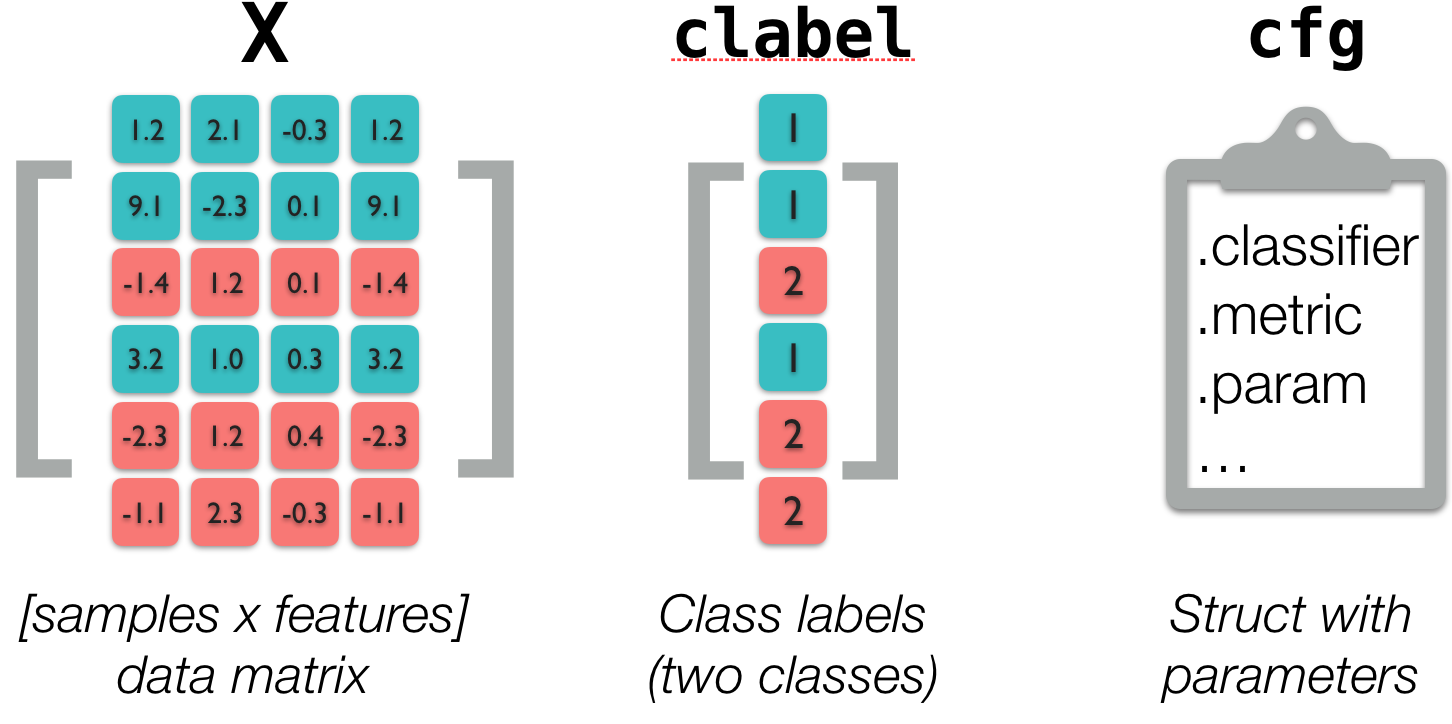
\includegraphics[width=.6\linewidth]{X_clabel_cfg}
% \caption{The three most commonly used input arguments in MVPA-Light. Colours are used to represent the two classes 1 (turquoise) and 2 (red) for illustrative purposes. Note that \textbf{X} can be three-dimensional (e.g. if it also has a time dimension) or even higher-dimensional (e.g. time-frequency data).}\label{fig:X}
% \end{figure}

\begin{figure}[ht!]
\centering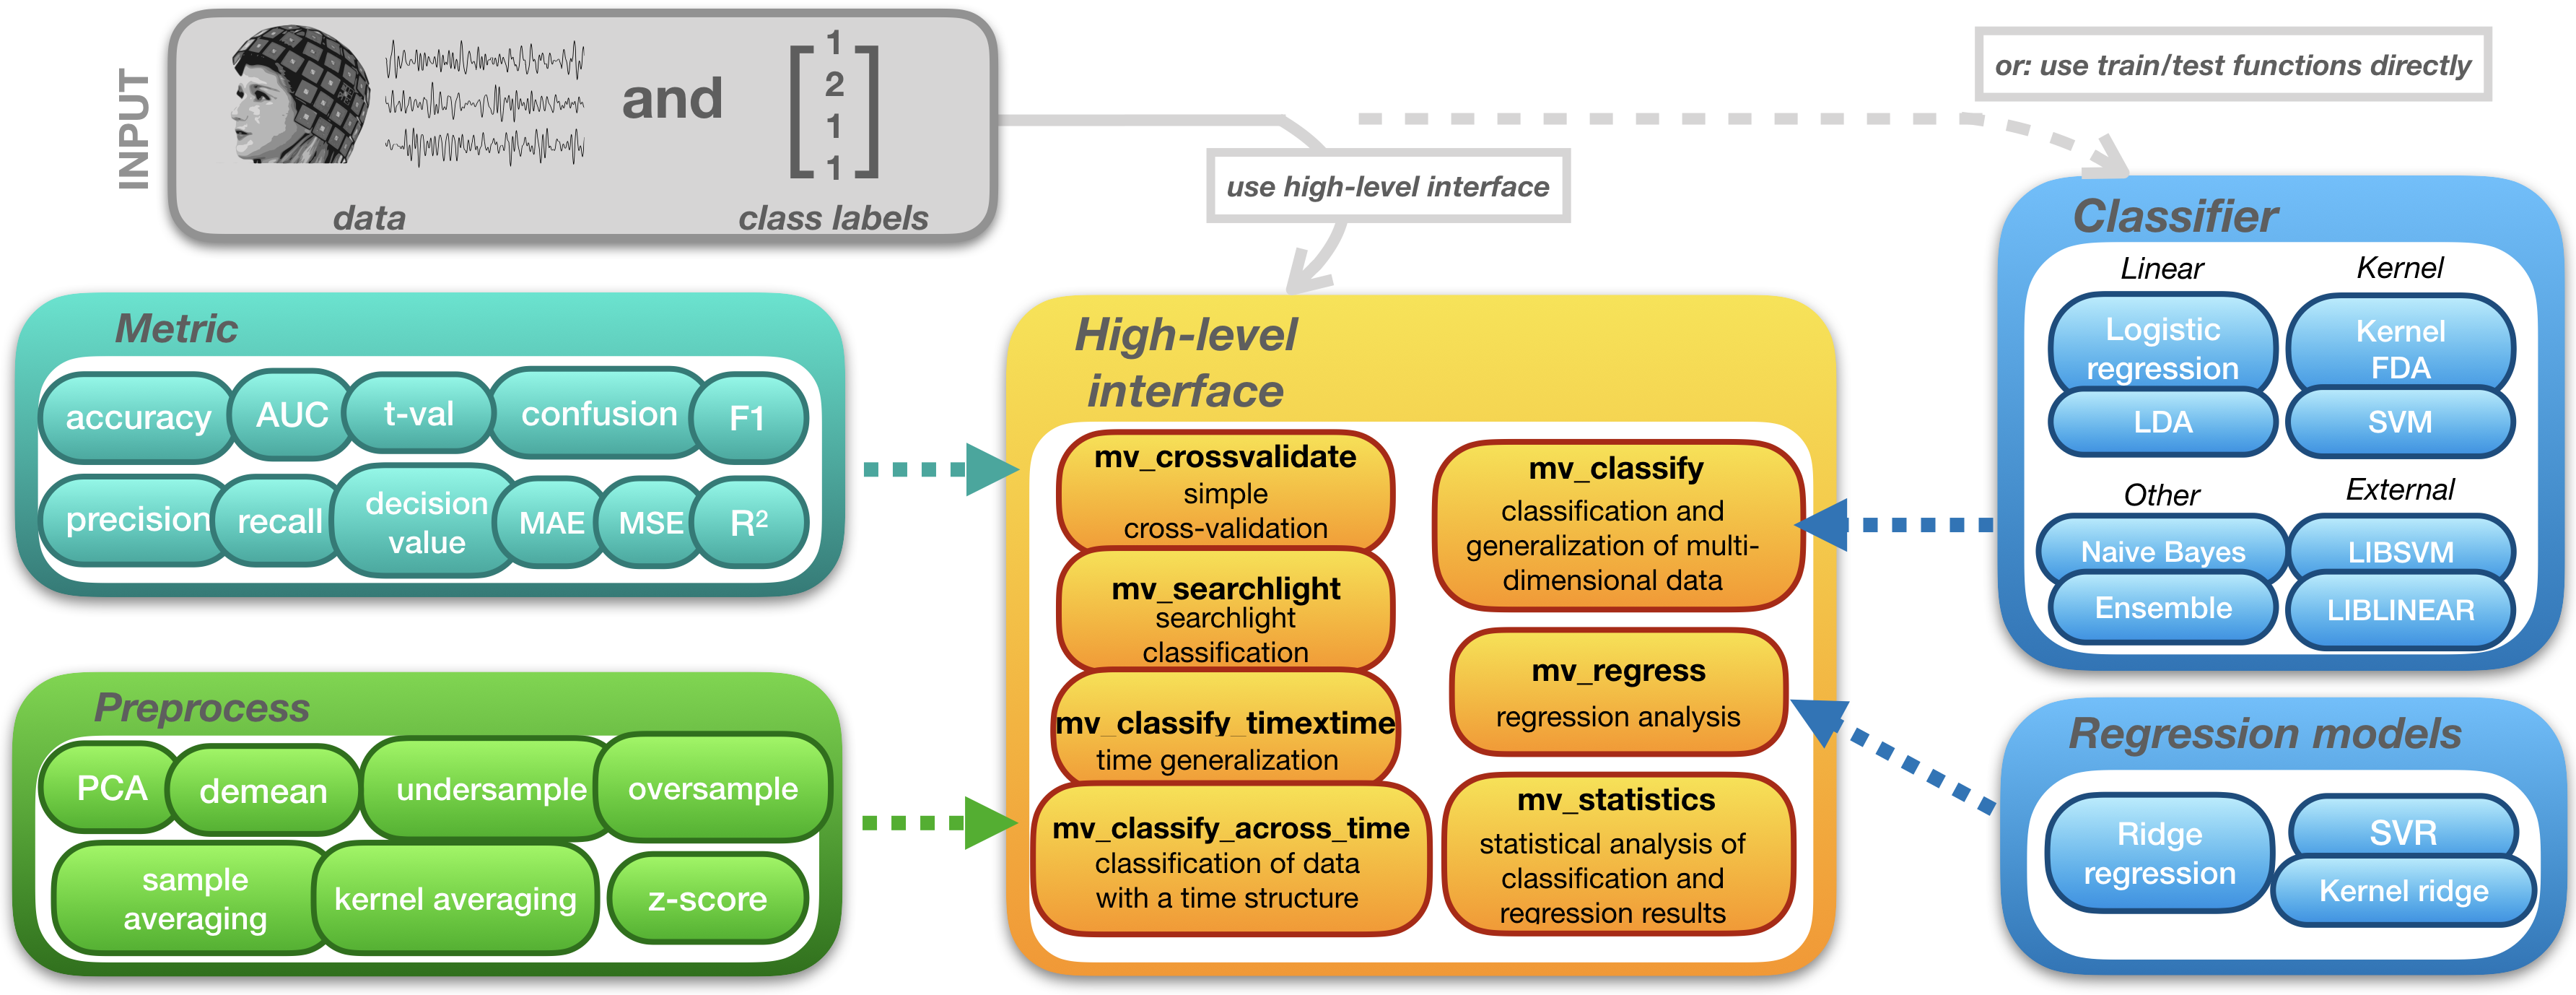
\includegraphics[width=\linewidth]{fig1_MVPA_structure}
\caption{Structure of MVPA-Light.}\label{fig:structure}
\end{figure}

\begin{figure}[ht!]
\centering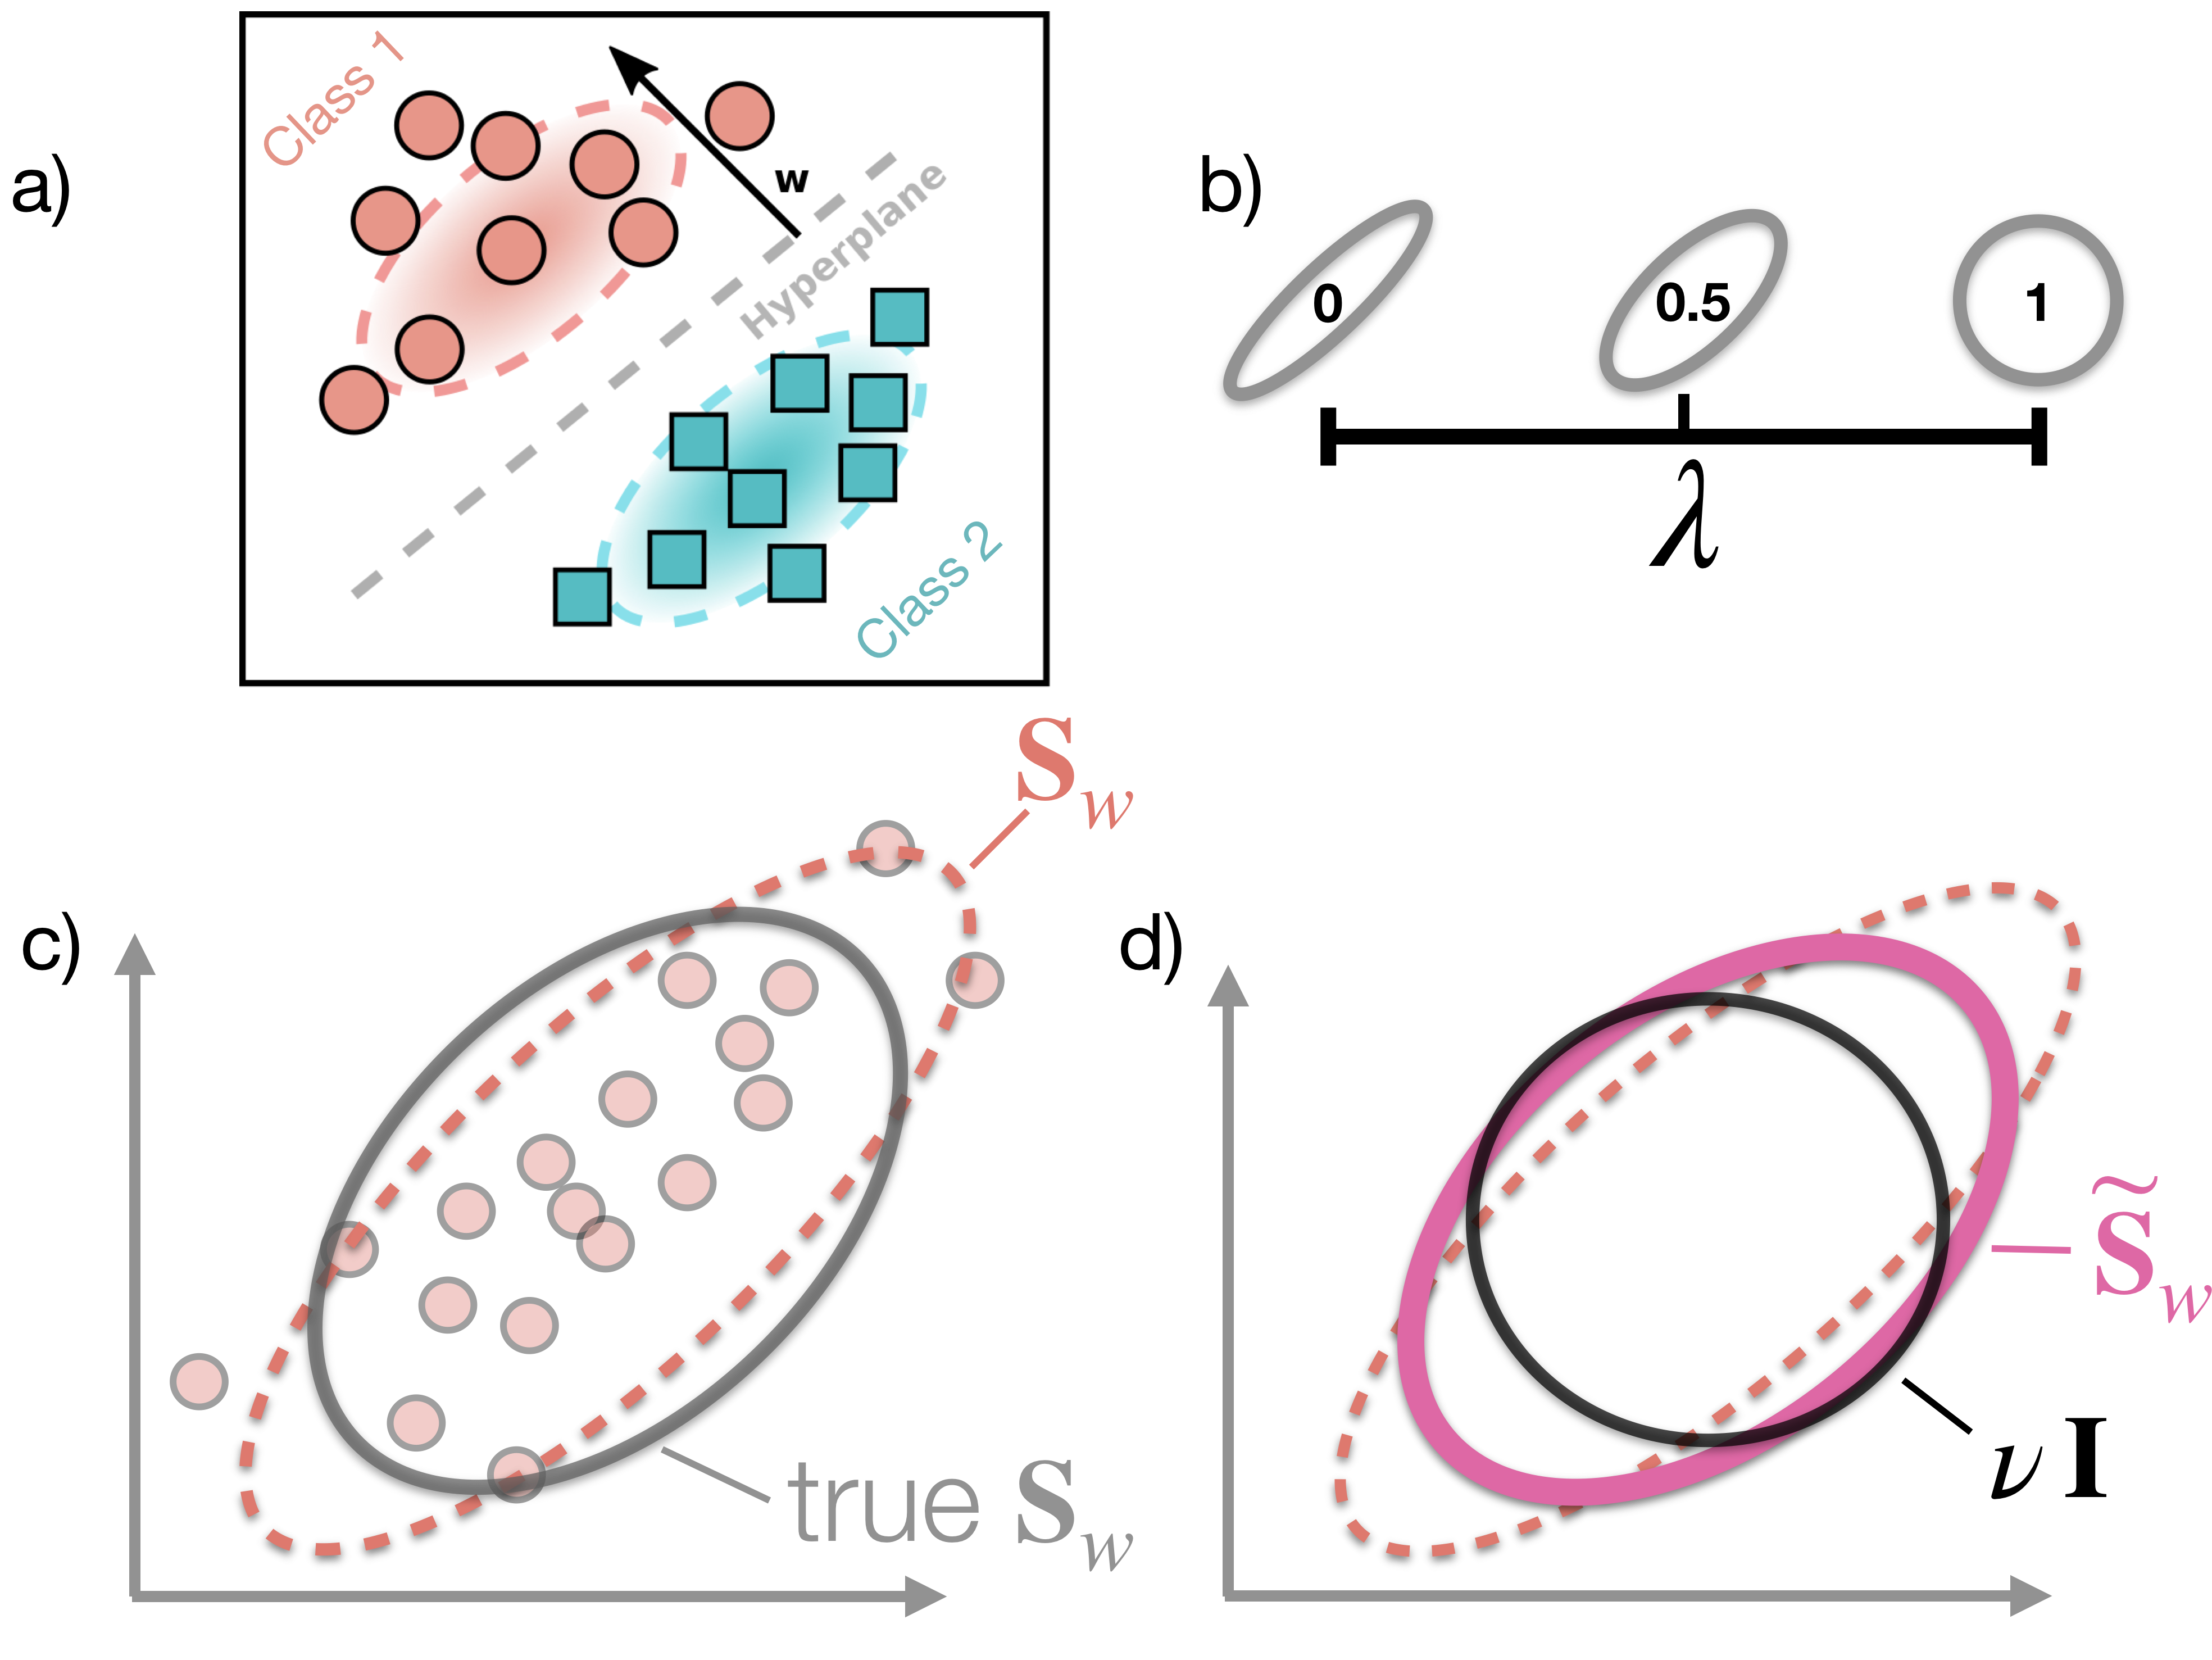
\includegraphics[width=\linewidth]{figures/LDA_regularization}
\caption{a) LDA with two classes. Covariance matrices are indicated by ellipses. The weight vector $\w$ is the normal to the hyperplane. b) Effect of varying $\lambda$ on the shape of the covariance matrix. c) Covariance matrices estimated from data usually overestimate large eigenvalues \citep{Blankertz2011}. d) The shrinkage estimate $\widetilde{\S}_w$ partially corrects the estimation error by shrinking towards a spherical covariance $\nu\mathbf{I}$.}\label{fig:lda}
\end{figure}

\begin{figure}[ht!]
\centering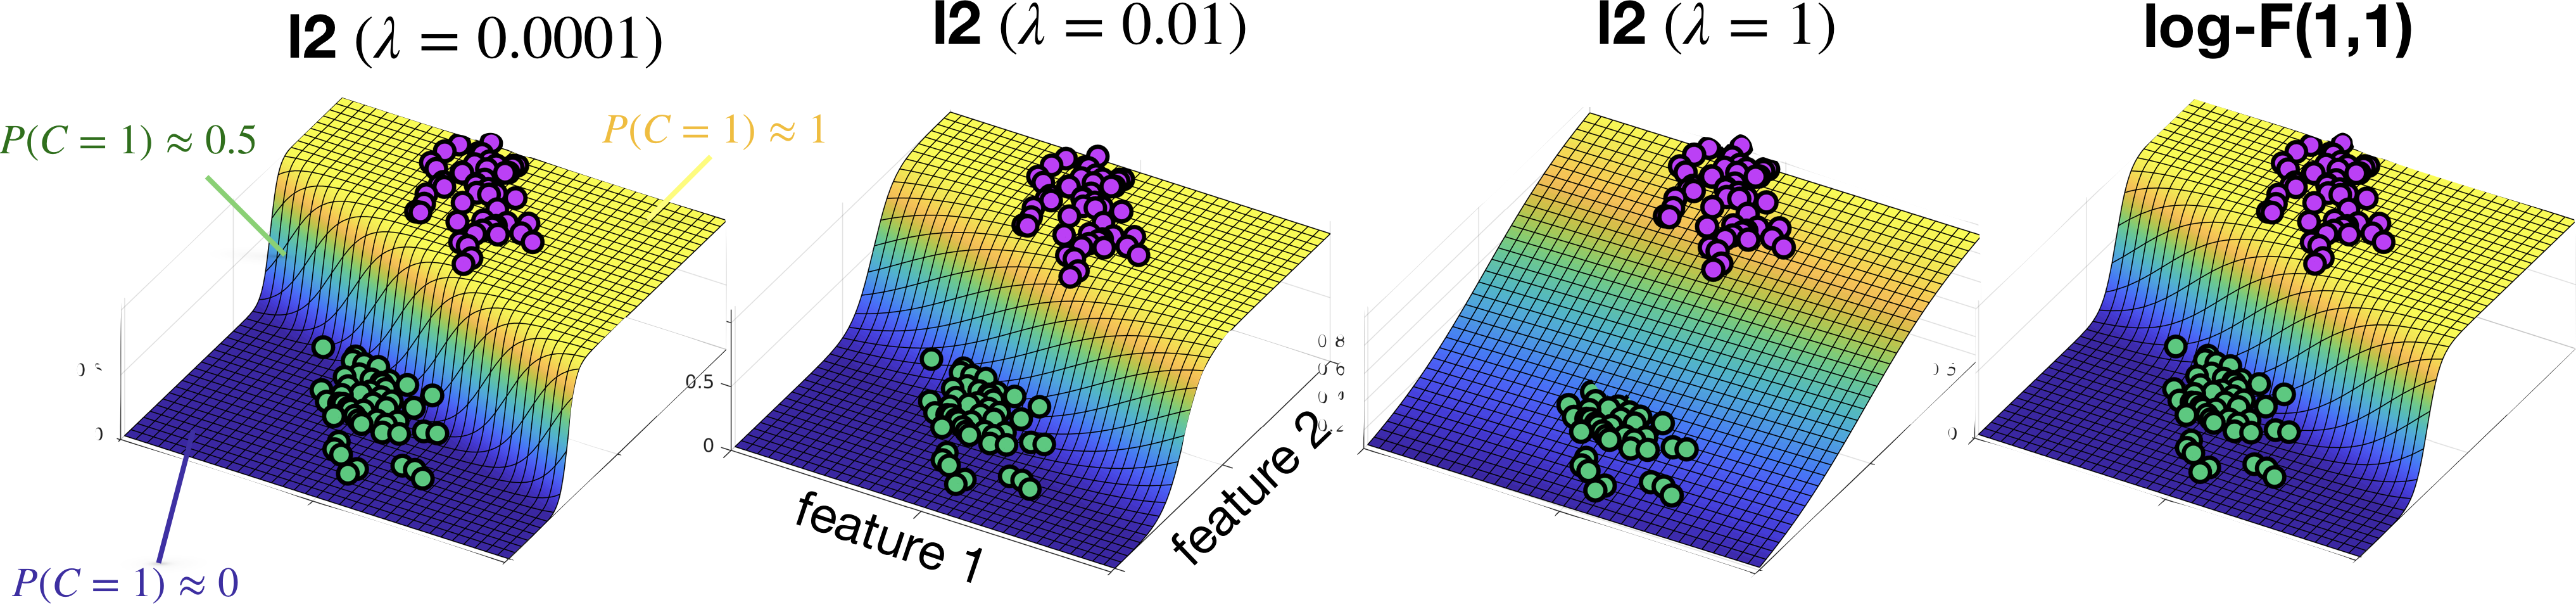
\includegraphics[width=\linewidth]{figures/logreg_regularization}
\caption{Logistic regression on data with two features (x and y axis) and two classes represented by purple (class 1) and green (class 2) dots. The curved surface is the sigmoid function fit and the vertical z-axis represents the probability for class 1. In L2 regularization, a larger $\lambda$ leads to a flatter sigmoid function with smoothly varying probabilities. For comparison, the sigmoid fit using Log-F(1,1) regularization is also shown.}\label{fig:logreg}
\end{figure}

\begin{figure}[ht!]
\centering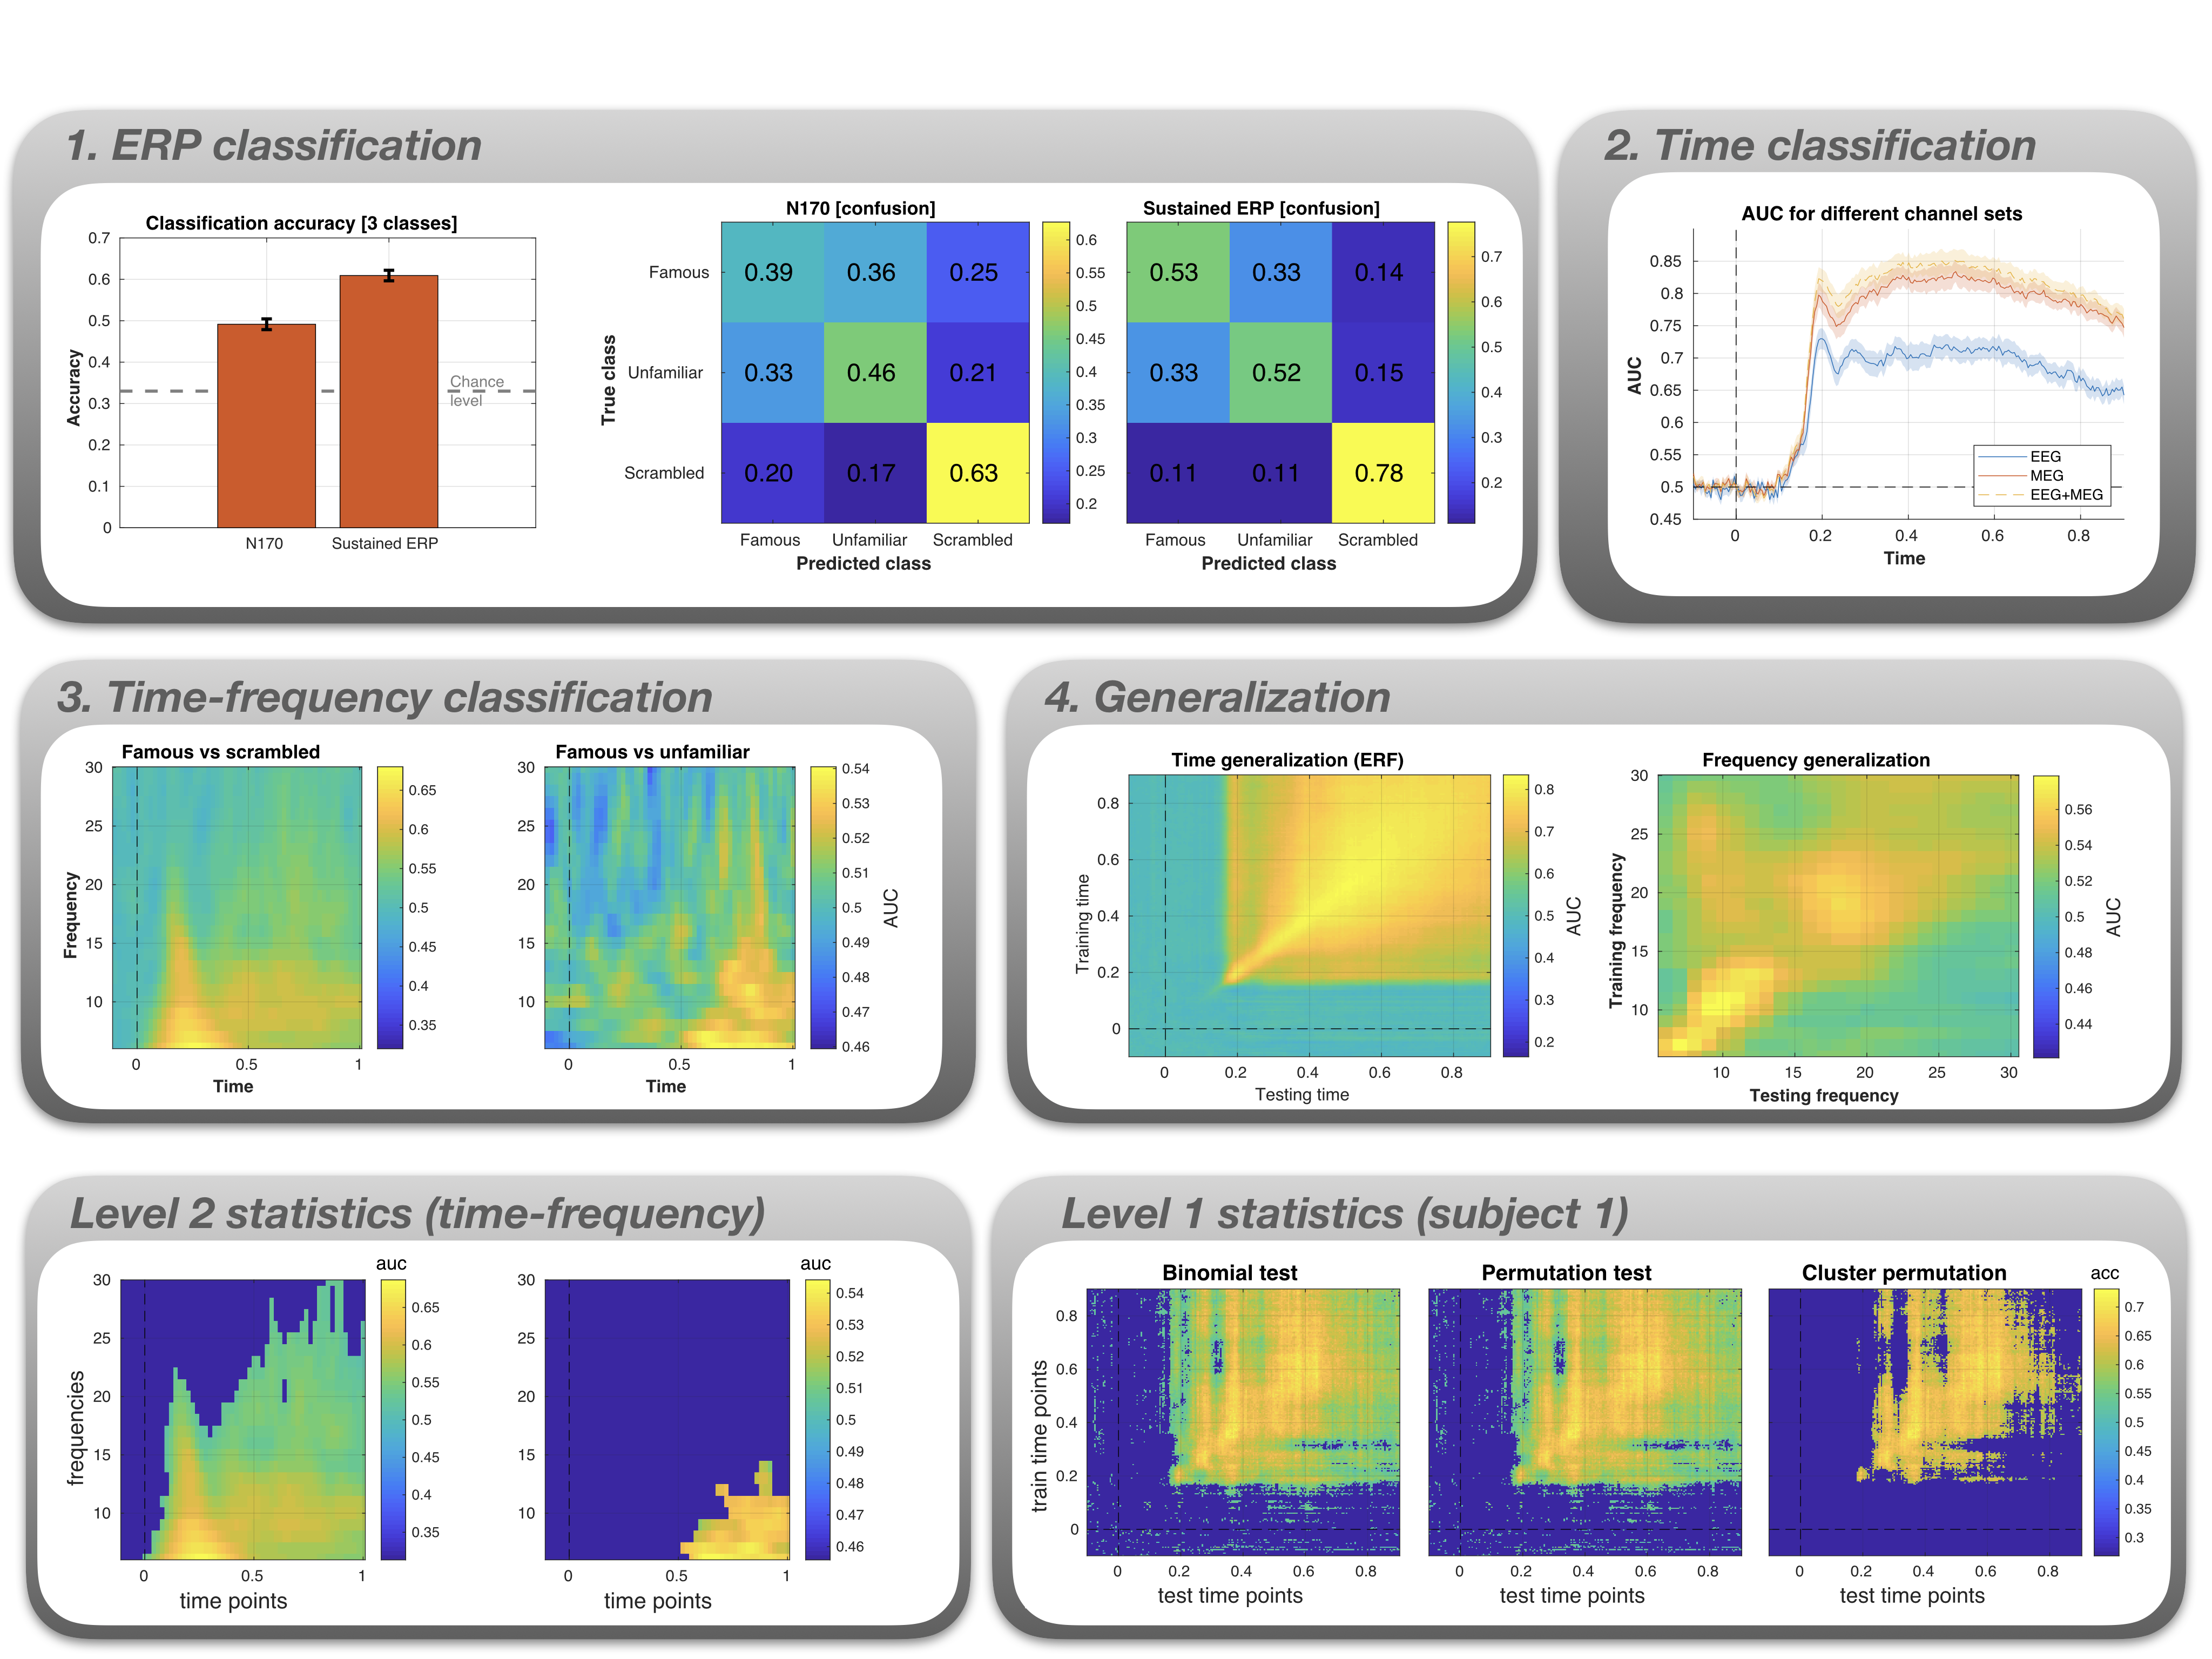
\includegraphics[width=\linewidth]{MVPA_results}
\caption{Results for the classification analysis of the \cite{Wakeman2015ADataset} MEEG data.}\label{fig:results}
\end{figure}


\begin{figure}[ht!]
\centering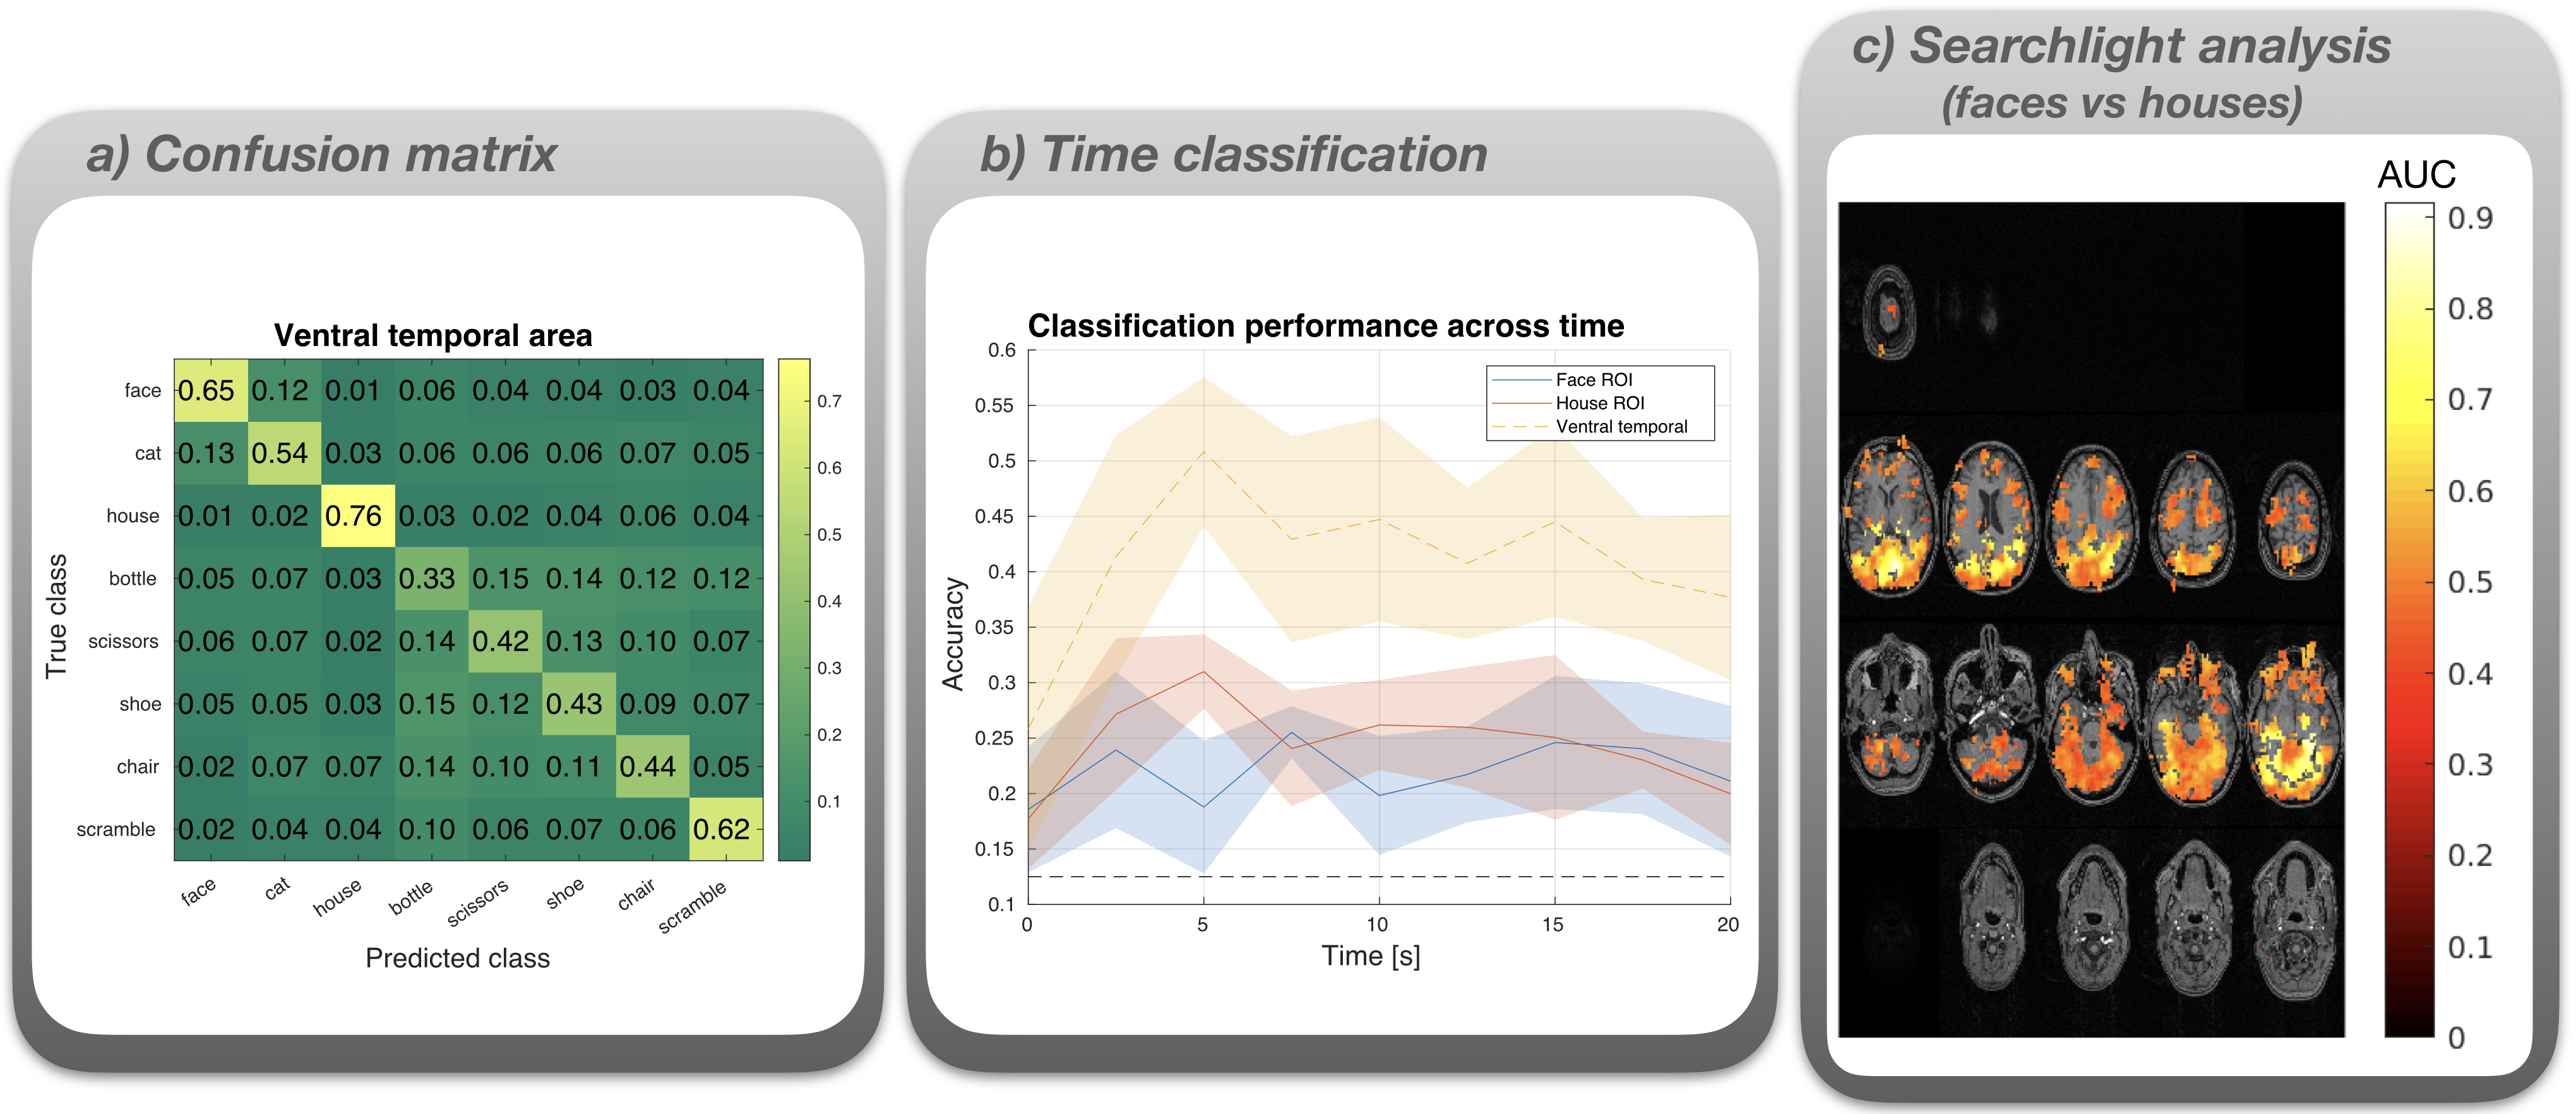
\includegraphics[width=\linewidth]{fmri_results}
\caption{Results for the classification analysis of the \cite{Haxby2001} fMRI data.}\label{fig:fmri_results}
\end{figure}

%%% If you are submitting a figure with subfigures please combine these into one image file with part labels integrated.
%%% If you don't add the figures in the LaTeX files, please upload them when submitting the article.
%%% Frontiers will add the figures at the end of the provisional pdf automatically
%%% The use of LaTeX coding to draw Diagrams/Figures/Structures should be avoided. They should be external callouts including graphics.

\end{document}
